
\documentclass[10pt]{article} % For LaTeX2e
\usepackage{tmlr}
% If accepted, instead use the following line for the camera-ready submission:
%\usepackage[accepted]{tmlr}
% To de-anonymize and remove mentions to TMLR (for example for posting to preprint servers), instead use the following:
%\usepackage[preprint]{tmlr}

% Optional math commands from https://github.com/goodfeli/dlbook_notation.
%%%%% NEW MATH DEFINITIONS %%%%%

\usepackage{amsmath,amsfonts,bm}

% Mark sections of captions for referring to divisions of figures
\newcommand{\figleft}{{\em (Left)}}
\newcommand{\figcenter}{{\em (Center)}}
\newcommand{\figright}{{\em (Right)}}
\newcommand{\figtop}{{\em (Top)}}
\newcommand{\figbottom}{{\em (Bottom)}}
\newcommand{\captiona}{{\em (a)}}
\newcommand{\captionb}{{\em (b)}}
\newcommand{\captionc}{{\em (c)}}
\newcommand{\captiond}{{\em (d)}}

% Highlight a newly defined term
\newcommand{\newterm}[1]{{\bf #1}}


% Figure reference, lower-case.
\def\figref#1{figure~\ref{#1}}
% Figure reference, capital. For start of sentence
\def\Figref#1{Figure~\ref{#1}}
\def\twofigref#1#2{figures \ref{#1} and \ref{#2}}
\def\quadfigref#1#2#3#4{figures \ref{#1}, \ref{#2}, \ref{#3} and \ref{#4}}
% Section reference, lower-case.
\def\secref#1{section~\ref{#1}}
% Section reference, capital.
\def\Secref#1{Section~\ref{#1}}
% Reference to two sections.
\def\twosecrefs#1#2{sections \ref{#1} and \ref{#2}}
% Reference to three sections.
\def\secrefs#1#2#3{sections \ref{#1}, \ref{#2} and \ref{#3}}
% Reference to an equation, lower-case.
\def\eqref#1{equation~\ref{#1}}
% Reference to an equation, upper case
\def\Eqref#1{Equation~\ref{#1}}
% A raw reference to an equation---avoid using if possible
\def\plaineqref#1{\ref{#1}}
% Reference to a chapter, lower-case.
\def\chapref#1{chapter~\ref{#1}}
% Reference to an equation, upper case.
\def\Chapref#1{Chapter~\ref{#1}}
% Reference to a range of chapters
\def\rangechapref#1#2{chapters\ref{#1}--\ref{#2}}
% Reference to an algorithm, lower-case.
\def\algref#1{algorithm~\ref{#1}}
% Reference to an algorithm, upper case.
\def\Algref#1{Algorithm~\ref{#1}}
\def\twoalgref#1#2{algorithms \ref{#1} and \ref{#2}}
\def\Twoalgref#1#2{Algorithms \ref{#1} and \ref{#2}}
% Reference to a part, lower case
\def\partref#1{part~\ref{#1}}
% Reference to a part, upper case
\def\Partref#1{Part~\ref{#1}}
\def\twopartref#1#2{parts \ref{#1} and \ref{#2}}

\def\ceil#1{\lceil #1 \rceil}
\def\floor#1{\lfloor #1 \rfloor}
\def\1{\bm{1}}
\newcommand{\train}{\mathcal{D}}
\newcommand{\valid}{\mathcal{D_{\mathrm{valid}}}}
\newcommand{\test}{\mathcal{D_{\mathrm{test}}}}

\def\eps{{\epsilon}}


% Random variables
\def\reta{{\textnormal{$\eta$}}}
\def\ra{{\textnormal{a}}}
\def\rb{{\textnormal{b}}}
\def\rc{{\textnormal{c}}}
\def\rd{{\textnormal{d}}}
\def\re{{\textnormal{e}}}
\def\rf{{\textnormal{f}}}
\def\rg{{\textnormal{g}}}
\def\rh{{\textnormal{h}}}
\def\ri{{\textnormal{i}}}
\def\rj{{\textnormal{j}}}
\def\rk{{\textnormal{k}}}
\def\rl{{\textnormal{l}}}
% rm is already a command, just don't name any random variables m
\def\rn{{\textnormal{n}}}
\def\ro{{\textnormal{o}}}
\def\rp{{\textnormal{p}}}
\def\rq{{\textnormal{q}}}
\def\rr{{\textnormal{r}}}
\def\rs{{\textnormal{s}}}
\def\rt{{\textnormal{t}}}
\def\ru{{\textnormal{u}}}
\def\rv{{\textnormal{v}}}
\def\rw{{\textnormal{w}}}
\def\rx{{\textnormal{x}}}
\def\ry{{\textnormal{y}}}
\def\rz{{\textnormal{z}}}

% Random vectors
\def\rvepsilon{{\mathbf{\epsilon}}}
\def\rvtheta{{\mathbf{\theta}}}
\def\rva{{\mathbf{a}}}
\def\rvb{{\mathbf{b}}}
\def\rvc{{\mathbf{c}}}
\def\rvd{{\mathbf{d}}}
\def\rve{{\mathbf{e}}}
\def\rvf{{\mathbf{f}}}
\def\rvg{{\mathbf{g}}}
\def\rvh{{\mathbf{h}}}
\def\rvu{{\mathbf{i}}}
\def\rvj{{\mathbf{j}}}
\def\rvk{{\mathbf{k}}}
\def\rvl{{\mathbf{l}}}
\def\rvm{{\mathbf{m}}}
\def\rvn{{\mathbf{n}}}
\def\rvo{{\mathbf{o}}}
\def\rvp{{\mathbf{p}}}
\def\rvq{{\mathbf{q}}}
\def\rvr{{\mathbf{r}}}
\def\rvs{{\mathbf{s}}}
\def\rvt{{\mathbf{t}}}
\def\rvu{{\mathbf{u}}}
\def\rvv{{\mathbf{v}}}
\def\rvw{{\mathbf{w}}}
\def\rvx{{\mathbf{x}}}
\def\rvy{{\mathbf{y}}}
\def\rvz{{\mathbf{z}}}

% Elements of random vectors
\def\erva{{\textnormal{a}}}
\def\ervb{{\textnormal{b}}}
\def\ervc{{\textnormal{c}}}
\def\ervd{{\textnormal{d}}}
\def\erve{{\textnormal{e}}}
\def\ervf{{\textnormal{f}}}
\def\ervg{{\textnormal{g}}}
\def\ervh{{\textnormal{h}}}
\def\ervi{{\textnormal{i}}}
\def\ervj{{\textnormal{j}}}
\def\ervk{{\textnormal{k}}}
\def\ervl{{\textnormal{l}}}
\def\ervm{{\textnormal{m}}}
\def\ervn{{\textnormal{n}}}
\def\ervo{{\textnormal{o}}}
\def\ervp{{\textnormal{p}}}
\def\ervq{{\textnormal{q}}}
\def\ervr{{\textnormal{r}}}
\def\ervs{{\textnormal{s}}}
\def\ervt{{\textnormal{t}}}
\def\ervu{{\textnormal{u}}}
\def\ervv{{\textnormal{v}}}
\def\ervw{{\textnormal{w}}}
\def\ervx{{\textnormal{x}}}
\def\ervy{{\textnormal{y}}}
\def\ervz{{\textnormal{z}}}

% Random matrices
\def\rmA{{\mathbf{A}}}
\def\rmB{{\mathbf{B}}}
\def\rmC{{\mathbf{C}}}
\def\rmD{{\mathbf{D}}}
\def\rmE{{\mathbf{E}}}
\def\rmF{{\mathbf{F}}}
\def\rmG{{\mathbf{G}}}
\def\rmH{{\mathbf{H}}}
\def\rmI{{\mathbf{I}}}
\def\rmJ{{\mathbf{J}}}
\def\rmK{{\mathbf{K}}}
\def\rmL{{\mathbf{L}}}
\def\rmM{{\mathbf{M}}}
\def\rmN{{\mathbf{N}}}
\def\rmO{{\mathbf{O}}}
\def\rmP{{\mathbf{P}}}
\def\rmQ{{\mathbf{Q}}}
\def\rmR{{\mathbf{R}}}
\def\rmS{{\mathbf{S}}}
\def\rmT{{\mathbf{T}}}
\def\rmU{{\mathbf{U}}}
\def\rmV{{\mathbf{V}}}
\def\rmW{{\mathbf{W}}}
\def\rmX{{\mathbf{X}}}
\def\rmY{{\mathbf{Y}}}
\def\rmZ{{\mathbf{Z}}}

% Elements of random matrices
\def\ermA{{\textnormal{A}}}
\def\ermB{{\textnormal{B}}}
\def\ermC{{\textnormal{C}}}
\def\ermD{{\textnormal{D}}}
\def\ermE{{\textnormal{E}}}
\def\ermF{{\textnormal{F}}}
\def\ermG{{\textnormal{G}}}
\def\ermH{{\textnormal{H}}}
\def\ermI{{\textnormal{I}}}
\def\ermJ{{\textnormal{J}}}
\def\ermK{{\textnormal{K}}}
\def\ermL{{\textnormal{L}}}
\def\ermM{{\textnormal{M}}}
\def\ermN{{\textnormal{N}}}
\def\ermO{{\textnormal{O}}}
\def\ermP{{\textnormal{P}}}
\def\ermQ{{\textnormal{Q}}}
\def\ermR{{\textnormal{R}}}
\def\ermS{{\textnormal{S}}}
\def\ermT{{\textnormal{T}}}
\def\ermU{{\textnormal{U}}}
\def\ermV{{\textnormal{V}}}
\def\ermW{{\textnormal{W}}}
\def\ermX{{\textnormal{X}}}
\def\ermY{{\textnormal{Y}}}
\def\ermZ{{\textnormal{Z}}}

% Vectors
\def\vzero{{\bm{0}}}
\def\vone{{\bm{1}}}
\def\vmu{{\bm{\mu}}}
\def\vtheta{{\bm{\theta}}}
\def\va{{\bm{a}}}
\def\vb{{\bm{b}}}
\def\vc{{\bm{c}}}
\def\vd{{\bm{d}}}
\def\ve{{\bm{e}}}
\def\vf{{\bm{f}}}
\def\vg{{\bm{g}}}
\def\vh{{\bm{h}}}
\def\vi{{\bm{i}}}
\def\vj{{\bm{j}}}
\def\vk{{\bm{k}}}
\def\vl{{\bm{l}}}
\def\vm{{\bm{m}}}
\def\vn{{\bm{n}}}
\def\vo{{\bm{o}}}
\def\vp{{\bm{p}}}
\def\vq{{\bm{q}}}
\def\vr{{\bm{r}}}
\def\vs{{\bm{s}}}
\def\vt{{\bm{t}}}
\def\vu{{\bm{u}}}
\def\vv{{\bm{v}}}
\def\vw{{\bm{w}}}
\def\vx{{\bm{x}}}
\def\vy{{\bm{y}}}
\def\vz{{\bm{z}}}

% Elements of vectors
\def\evalpha{{\alpha}}
\def\evbeta{{\beta}}
\def\evepsilon{{\epsilon}}
\def\evlambda{{\lambda}}
\def\evomega{{\omega}}
\def\evmu{{\mu}}
\def\evpsi{{\psi}}
\def\evsigma{{\sigma}}
\def\evtheta{{\theta}}
\def\eva{{a}}
\def\evb{{b}}
\def\evc{{c}}
\def\evd{{d}}
\def\eve{{e}}
\def\evf{{f}}
\def\evg{{g}}
\def\evh{{h}}
\def\evi{{i}}
\def\evj{{j}}
\def\evk{{k}}
\def\evl{{l}}
\def\evm{{m}}
\def\evn{{n}}
\def\evo{{o}}
\def\evp{{p}}
\def\evq{{q}}
\def\evr{{r}}
\def\evs{{s}}
\def\evt{{t}}
\def\evu{{u}}
\def\evv{{v}}
\def\evw{{w}}
\def\evx{{x}}
\def\evy{{y}}
\def\evz{{z}}

% Matrix
\def\mA{{\bm{A}}}
\def\mB{{\bm{B}}}
\def\mC{{\bm{C}}}
\def\mD{{\bm{D}}}
\def\mE{{\bm{E}}}
\def\mF{{\bm{F}}}
\def\mG{{\bm{G}}}
\def\mH{{\bm{H}}}
\def\mI{{\bm{I}}}
\def\mJ{{\bm{J}}}
\def\mK{{\bm{K}}}
\def\mL{{\bm{L}}}
\def\mM{{\bm{M}}}
\def\mN{{\bm{N}}}
\def\mO{{\bm{O}}}
\def\mP{{\bm{P}}}
\def\mQ{{\bm{Q}}}
\def\mR{{\bm{R}}}
\def\mS{{\bm{S}}}
\def\mT{{\bm{T}}}
\def\mU{{\bm{U}}}
\def\mV{{\bm{V}}}
\def\mW{{\bm{W}}}
\def\mX{{\bm{X}}}
\def\mY{{\bm{Y}}}
\def\mZ{{\bm{Z}}}
\def\mBeta{{\bm{\beta}}}
\def\mPhi{{\bm{\Phi}}}
\def\mLambda{{\bm{\Lambda}}}
\def\mSigma{{\bm{\Sigma}}}

% Tensor
\DeclareMathAlphabet{\mathsfit}{\encodingdefault}{\sfdefault}{m}{sl}
\SetMathAlphabet{\mathsfit}{bold}{\encodingdefault}{\sfdefault}{bx}{n}
\newcommand{\tens}[1]{\bm{\mathsfit{#1}}}
\def\tA{{\tens{A}}}
\def\tB{{\tens{B}}}
\def\tC{{\tens{C}}}
\def\tD{{\tens{D}}}
\def\tE{{\tens{E}}}
\def\tF{{\tens{F}}}
\def\tG{{\tens{G}}}
\def\tH{{\tens{H}}}
\def\tI{{\tens{I}}}
\def\tJ{{\tens{J}}}
\def\tK{{\tens{K}}}
\def\tL{{\tens{L}}}
\def\tM{{\tens{M}}}
\def\tN{{\tens{N}}}
\def\tO{{\tens{O}}}
\def\tP{{\tens{P}}}
\def\tQ{{\tens{Q}}}
\def\tR{{\tens{R}}}
\def\tS{{\tens{S}}}
\def\tT{{\tens{T}}}
\def\tU{{\tens{U}}}
\def\tV{{\tens{V}}}
\def\tW{{\tens{W}}}
\def\tX{{\tens{X}}}
\def\tY{{\tens{Y}}}
\def\tZ{{\tens{Z}}}


% Graph
\def\gA{{\mathcal{A}}}
\def\gB{{\mathcal{B}}}
\def\gC{{\mathcal{C}}}
\def\gD{{\mathcal{D}}}
\def\gE{{\mathcal{E}}}
\def\gF{{\mathcal{F}}}
\def\gG{{\mathcal{G}}}
\def\gH{{\mathcal{H}}}
\def\gI{{\mathcal{I}}}
\def\gJ{{\mathcal{J}}}
\def\gK{{\mathcal{K}}}
\def\gL{{\mathcal{L}}}
\def\gM{{\mathcal{M}}}
\def\gN{{\mathcal{N}}}
\def\gO{{\mathcal{O}}}
\def\gP{{\mathcal{P}}}
\def\gQ{{\mathcal{Q}}}
\def\gR{{\mathcal{R}}}
\def\gS{{\mathcal{S}}}
\def\gT{{\mathcal{T}}}
\def\gU{{\mathcal{U}}}
\def\gV{{\mathcal{V}}}
\def\gW{{\mathcal{W}}}
\def\gX{{\mathcal{X}}}
\def\gY{{\mathcal{Y}}}
\def\gZ{{\mathcal{Z}}}

% Sets
\def\sA{{\mathbb{A}}}
\def\sB{{\mathbb{B}}}
\def\sC{{\mathbb{C}}}
\def\sD{{\mathbb{D}}}
% Don't use a set called E, because this would be the same as our symbol
% for expectation.
\def\sF{{\mathbb{F}}}
\def\sG{{\mathbb{G}}}
\def\sH{{\mathbb{H}}}
\def\sI{{\mathbb{I}}}
\def\sJ{{\mathbb{J}}}
\def\sK{{\mathbb{K}}}
\def\sL{{\mathbb{L}}}
\def\sM{{\mathbb{M}}}
\def\sN{{\mathbb{N}}}
\def\sO{{\mathbb{O}}}
\def\sP{{\mathbb{P}}}
\def\sQ{{\mathbb{Q}}}
\def\sR{{\mathbb{R}}}
\def\sS{{\mathbb{S}}}
\def\sT{{\mathbb{T}}}
\def\sU{{\mathbb{U}}}
\def\sV{{\mathbb{V}}}
\def\sW{{\mathbb{W}}}
\def\sX{{\mathbb{X}}}
\def\sY{{\mathbb{Y}}}
\def\sZ{{\mathbb{Z}}}

% Entries of a matrix
\def\emLambda{{\Lambda}}
\def\emA{{A}}
\def\emB{{B}}
\def\emC{{C}}
\def\emD{{D}}
\def\emE{{E}}
\def\emF{{F}}
\def\emG{{G}}
\def\emH{{H}}
\def\emI{{I}}
\def\emJ{{J}}
\def\emK{{K}}
\def\emL{{L}}
\def\emM{{M}}
\def\emN{{N}}
\def\emO{{O}}
\def\emP{{P}}
\def\emQ{{Q}}
\def\emR{{R}}
\def\emS{{S}}
\def\emT{{T}}
\def\emU{{U}}
\def\emV{{V}}
\def\emW{{W}}
\def\emX{{X}}
\def\emY{{Y}}
\def\emZ{{Z}}
\def\emSigma{{\Sigma}}

% entries of a tensor
% Same font as tensor, without \bm wrapper
\newcommand{\etens}[1]{\mathsfit{#1}}
\def\etLambda{{\etens{\Lambda}}}
\def\etA{{\etens{A}}}
\def\etB{{\etens{B}}}
\def\etC{{\etens{C}}}
\def\etD{{\etens{D}}}
\def\etE{{\etens{E}}}
\def\etF{{\etens{F}}}
\def\etG{{\etens{G}}}
\def\etH{{\etens{H}}}
\def\etI{{\etens{I}}}
\def\etJ{{\etens{J}}}
\def\etK{{\etens{K}}}
\def\etL{{\etens{L}}}
\def\etM{{\etens{M}}}
\def\etN{{\etens{N}}}
\def\etO{{\etens{O}}}
\def\etP{{\etens{P}}}
\def\etQ{{\etens{Q}}}
\def\etR{{\etens{R}}}
\def\etS{{\etens{S}}}
\def\etT{{\etens{T}}}
\def\etU{{\etens{U}}}
\def\etV{{\etens{V}}}
\def\etW{{\etens{W}}}
\def\etX{{\etens{X}}}
\def\etY{{\etens{Y}}}
\def\etZ{{\etens{Z}}}

% The true underlying data generating distribution
\newcommand{\pdata}{p_{\rm{data}}}
% The empirical distribution defined by the training set
\newcommand{\ptrain}{\hat{p}_{\rm{data}}}
\newcommand{\Ptrain}{\hat{P}_{\rm{data}}}
% The model distribution
\newcommand{\pmodel}{p_{\rm{model}}}
\newcommand{\Pmodel}{P_{\rm{model}}}
\newcommand{\ptildemodel}{\tilde{p}_{\rm{model}}}
% Stochastic autoencoder distributions
\newcommand{\pencode}{p_{\rm{encoder}}}
\newcommand{\pdecode}{p_{\rm{decoder}}}
\newcommand{\precons}{p_{\rm{reconstruct}}}

\newcommand{\laplace}{\mathrm{Laplace}} % Laplace distribution

\newcommand{\E}{\mathbb{E}}
\newcommand{\Ls}{\mathcal{L}}
\newcommand{\R}{\mathbb{R}}
\newcommand{\emp}{\tilde{p}}
\newcommand{\lr}{\alpha}
\newcommand{\reg}{\lambda}
\newcommand{\rect}{\mathrm{rectifier}}
\newcommand{\softmax}{\mathrm{softmax}}
\newcommand{\sigmoid}{\sigma}
\newcommand{\softplus}{\zeta}
\newcommand{\KL}{D_{\mathrm{KL}}}
\newcommand{\Var}{\mathrm{Var}}
\newcommand{\standarderror}{\mathrm{SE}}
\newcommand{\Cov}{\mathrm{Cov}}
% Wolfram Mathworld says $L^2$ is for function spaces and $\ell^2$ is for vectors
% But then they seem to use $L^2$ for vectors throughout the site, and so does
% wikipedia.
\newcommand{\normlzero}{L^0}
\newcommand{\normlone}{L^1}
\newcommand{\normltwo}{L^2}
\newcommand{\normlp}{L^p}
\newcommand{\normmax}{L^\infty}

\newcommand{\parents}{Pa} % See usage in notation.tex. Chosen to match Daphne's book.

\DeclareMathOperator*{\argmax}{arg\,max}
\DeclareMathOperator*{\argmin}{arg\,min}

\DeclareMathOperator{\sign}{sign}
\DeclareMathOperator{\Tr}{Tr}
\let\ab\allowbreak


\usepackage{hyperref}
\usepackage{url}
\usepackage{amssymb}
\usepackage{amsthm}
\usepackage{booktabs}
\usepackage{graphicx}
\usepackage{multirow}


% Custom commands
\newtheorem{proposition}{Proposition}
\newcommand{\K}{\mathbf{K}}
\newcommand{\B}{\mathbf{B}}
\newcommand{\z}{\bm{z}}
\newcommand{\x}{\bm{x}}

\title{Bounded Is Not Better:\\ Trivial Baselines and Scale Confounds in Latent World-Model Evaluation}

% Authors must not appear in the submitted version. They should be hidden
% as long as the tmlr package is used without the [accepted] or [preprint] options.
% Non-anonymous submissions will be rejected without review.

\author{\name Pascal J. Sager \email sage@zhaw.ch \\
      \addr Centre for Artificial Intelligence\\
      Zurich University of Applied Sciences\\
      Technikumstrasse 71, 8400 Winterthur, Switzerland
      \AND
      \name Yassine Taoudi-Benchekroun \email ytaoudi@ethz.ch \\
      \addr Institute of Neuroinformatics\\
      University of Zurich and ETH Zurich\\
      Winterthurerstrasse 190, 8057 Zurich, Switzerland
      \AND
      \name Benjamin F. Grewe \email bgrewe@ethz.ch \\
      \addr Institute of Neuroinformatics\\
      University of Zurich and ETH Zurich\\
      Winterthurerstrasse 190, 8057 Zurich, Switzerland
      \AND
      \name Thilo Stadelmann \email stdm@zhaw.ch \\
      \addr Centre for Artificial Intelligence\\
      Zurich University of Applied Sciences\\
      Technikumstrasse 71, 8400 Winterthur, Switzerland}

% The \author macro works with any number of authors. Use \AND 
% to separate the names and addresses of multiple authors.


\def\month{MM}  % Insert correct month for camera-ready version
\def\year{YYYY} % Insert correct year for camera-ready version
\def\openreview{\url{https://openreview.net/forum?id=XXXX}} % Insert correct link to OpenReview for camera-ready version


\begin{document}

\maketitle

\begin{abstract}
% [new] DONE. No coined vocabulary and no emphasis: the two trivial predictors
% and the second readout are described rather than named, because the reader
% has nowhere to look a name up. Ends on the paper's one sentence.
World models predict how a latent state evolves under actions, and multi-step prediction feeds the model's output back into itself, so per-step error compounds. A known remedy constrains the latent transition operator so it cannot amplify error, replacing exponential worst-case growth with linear. We test it under control: one encoder, one objective, four dynamics modules differing only in the spectral constraint, tuned independently, ten seeds, two environments.

Measured as this literature measures, with a probe from the latent to physical coordinates, the constraint works by five orders of magnitude. It does not survive two controls that cost one line each. Copying the current latent forward, or returning the training set's average state, beats every learned model in all $168$ cells we measure at ten steps and beyond. Scoring the same rollouts by matching each predicted latent to the nearest encoded held-out frame, which ignores vector length, shrinks those five orders of magnitude to a factor of $1.4$ without changing the ordering.

The cause is measurable. The probe is fitted at the scale of encoded observations and penalizes a rollout whose norm drifts, and the bound behind the constraint limits exactly that drift. The two agree by construction. We measure the drift, move it by rescaling a trained operator, and remove it by changing the prediction loss, which closes the gap and still leaves every model behind the trivial predictors. A bounded error curve under a scale-sensitive readout is a property of the constraint, not evidence of a learned model.
\end{abstract}


% =============================================================================
% LABEL MAP. Every label used in the approved paper (main) or in the
% evaluation-controls draft, and where it went. Checked by step 6.3.
%
%   approved / draft label      ->  this paper
%   --------------------------------------------------------------------------
%   sec:intro                   ->  sec:intro
%   sec:background              ->  sec:background
%   (new)                       ->  sec:koopman        2.1
%   (new)                       ->  sec:bound          2.2
%   sec:bound_limits  [draft]   ->  sec:bound_limits   2.3
%   sec:related                 ->  sec:related
%   sec:arch                    ->  sec:arch           section 4
%   (new)                       ->  sec:variants       4.1
%   (new)                       ->  sec:protocol       4.2
%   sec:measurements  [draft]   ->  sec:measurements   4.3
%   sec:exp                     ->  sec:exp            section 5
%   sec:results                 ->  sec:results        5.1
%   sec:inversion     [draft]   ->  sec:inversion      5.2
%   sec:spectrum      [draft]   ->  sec:spectrum       5.3
%   (new)                       ->  sec:loss           5.4
%   sec:degeneracy    [draft]   ->  sec:degeneracy     5.5
%   sec:checklist     [draft]   ->  sec:checklist      section 6
%   sec:limitations             ->  sec:limitations
%   sec:conclusion              ->  sec:conclusion
%   sec:soft                    ->  app:soft           appendix B
%   sec:cayley                  ->  app:dmd            appendix C
%   sec:outlook_lqr             ->  app:lqr            appendix D
%   sec:efficiency              ->  CUT (one line in appendix E)
%   sec:robustness              ->  CUT (one line in appendix E)
%   app:impl                    ->  app:impl           appendix A
%   app:dmd                     ->  app:dmd            appendix C
%   app:lqr                     ->  app:lqr            appendix D
%   app:full_results            ->  app:full_results   appendix E
%   (new)                       ->  app:drift          appendix F
%   app:provenance    [draft]   ->  app:provenance     appendix G
%   app:visual_mse              ->  CUT (one sentence in 5.2)
%   eq:compound                 ->  eq:compound
%   eq:koopman_def              ->  eq:koopman_def
%   eq:linear_bound             ->  eq:linear_bound
%   eq:base_loss                ->  eq:base_loss
%   eq:soft_penalty             ->  eq:soft_penalty    appendix B
%   eq:cayley                   ->  eq:cayley          appendix C
%   eq:dare                     ->  eq:dare            appendix D
%   eq:lqr_law                  ->  eq:lqr_law         appendix D
%   eq:error_dynamics           ->  eq:error_dynamics  appendix D
%   eq:soft_loss                ->  CUT (folded into eq:soft_penalty)
%   eq:steady_state   [draft]   ->  CUT
%   prop:cayley-stab            ->  prop:cayley-stab   appendix D
%   fig:architecture            ->  fig:architecture   figure 1
%   fig:rho_sweep     [draft]   ->  fig:rho_sweep      figure 2
%   fig:degeneracy    [draft]   ->  fig:degeneracy     figure 3
%   fig:compounding_controls    ->  fig:compounding_controls  appendix F
%   fig:eigenvalues             ->  fig:eigenvalues    appendix F
%   fig:environments            ->  fig:environments   appendix A
%   fig:compounding   [draft]   ->  CUT (superseded by fig:compounding_controls)
%   fig:data_efficiency         ->  CUT
%   fig:robustness              ->  CUT
%   tab:combined                ->  tab:combined       table 1
%   tab:retrieval     [draft]   ->  tab:retrieval      table 2
%   (new)                       ->  tab:l2_ablation    table 3
%   tab:control       [draft]   ->  tab:control        appendix D
%   (new)                       ->  tab:full_controls_pendulum   appendix E
%   (new)                       ->  tab:full_controls_cartpole   appendix E
%   tab:hyperparams             ->  tab:hyperparams    appendix A
%   tab:search_space            ->  tab:search_space   appendix A
%   tab:lqr                     ->  CUT (superseded by tab:control)
%   tab:full                    ->  CUT (superseded by tab:full_controls_*)
%   tab:data_efficiency         ->  CUT
%   tab:robustness              ->  CUT
%   tab:robustness_cartpole     ->  CUT
%   tab:visual_mse              ->  CUT
%   tab:provenance    [draft]   ->  CUT (appendix G is prose)
%
% SOURCE TAGS below: [orig] = approved text, carried over. [draft] = prose from
% the evaluation-controls branch. [new] = to be written. Word counts are the
% budget from PAPER_PLAN section 4, not a measurement.
% =============================================================================

\section{Introduction}
\label{sec:intro}
% [orig 1 p1] DONE, verbatim.
World models~\citep{Ha2018} encode observations into latent representations and predict how these representations evolve under action sequences, enabling autonomous agents to plan ahead by simulating future trajectories internally~\citep{schmidhuber1990making,Sager2025Agents}.
The dominant paradigm predicts latent transitions with feedforward networks or recurrent state-space models (RSSMs)~\citep{Hafner2019Planet,Hafner2025,Hansen2023}.
These models are expressive and effective at short horizons~\citep{Hansen2023}, but multi-step prediction requires feeding the dynamics model's output back into itself, so each per-step approximation error is propagated by every subsequent application of the map. Where the map is locally expanding, the worst-case error bound grows exponentially in the horizon (Section~\ref{sec:background}). This failure mode is well documented, and prior
work has mitigated it by training models on their own rollouts, by planning with temporally abstract models, and by learning value-equivalent latent dynamics (Section~\ref{sec:related}). We take a complementary route that constrains the structure of the transition operator itself.

% [orig 1 p2] DONE. Trimmed: stops before the JEPA justification, which now
% belongs to Section 4.1. Two changes to the approved wording. "additionally"
% is a banned filler word and is dropped, and the closing sentence points at
% Section 2.2 instead of running on into the architecture.
We address this by constraining the latent transition operator to be non-expansive, using Koopman operator theory~\citep{Koopman1931} as the framing. The theory is based on the insight that nonlinear observations can be lifted into a higher-dimensional feature space where the dynamics become strictly linear, provided the space is of sufficient (and potentially infinite) dimension.
In such an ideally linear regime, multi-step prediction reduces to a matrix power. If the matrix is also constrained so that it cannot amplify errors, error accumulates at most linearly rather than exponentially (Section~\ref{sec:bound}).
% [new 1 p3, p4] DONE. The pivot and the contributions, in prose.
We built the controlled comparison this argument calls for. One encoder, one objective, four dynamics modules differing only in how the spectrum of the transition operator is constrained, each tuned independently, ten seeds, two environments. Measured with a probe from the latent state to physical coordinates, which is the standard readout in this literature, the constraint works by five orders of magnitude. It does not survive two controls that cost one line each. A predictor that copies the current latent forward and a predictor that returns the dataset mean are more accurate than every learned model in all $168$ of the environment, background, data-fraction, module and horizon cells we measure at $T \ge 10$. The reason is structural. The probe is fitted at the scale of encoded observations and charges a rollout for leaving that scale. The error bound that motivates the constraint limits exactly how far a rollout can leave it. An operator satisfying the bound therefore scores well under the probe whether or not it has learned the dynamics.

This paper reports that study as an evaluation result. We show that a carefully controlled empirical separation between world-model architectures is produced by a confound rather than by the property under test. We then measure the confound rather than arguing for it, in four ways: pairing the probe with a readout that ignores latent scale, measuring norm growth on the learned operators directly, moving the spectrum of a trained operator and watching the metric follow, and removing the mismatch at its source with a different prediction loss. What survives is the mechanism the theory describes, that error growth tracks the spectral radius, rather than the architecture built to exploit it. We close with the five measurements that would have caught this, none of which needs a model to be retrained.

% =============================================================================
\section{Error Growth, and What a Spectral Bound Does Not Say}
\label{sec:background}

\subsection{Koopman Lifting Turns a Rollout into a Matrix Power}
\label{sec:koopman}
% [orig 2.1] DONE. Three paragraphs of the approved text compressed into two.
% Both footnotes kept, the second shortened. The Brunton citation on
% Koopman-invariant subspaces is kept because it is what makes the residual
% irreducible rather than a matter of width.
Let $\z_t \in \mathbb{R}^D$ be a latent representation of an environment at time step $t$, and let $f_\theta$ be a learned nonlinear transition model pointwise satisfying $\|f_\theta(\z) - f^*(\z)\| \le \epsilon$, where $f^*$ denotes the true latent space dynamics. To predict several steps ahead the model feeds its own output back into itself, and each application multiplies the accumulated error by the Lipschitz constant $L$ of the transition function\footnote{The Lipschitz constant $L$ of a function $f$ is the smallest value such that $\|f(\z) - f(\z')\| \le L\|\z - \z'\|$ for all inputs $\z, \z'$. It measures how much $f$ can stretch distances between inputs. If $L < 1$ the function contracts distances and small errors shrink at each step. If $L > 1$ the function stretches distances and small errors grow.}. For non-trivial physical dynamics $L > 1$ holds,\footnote{Even in globally dissipative systems the local Lipschitz constant exceeds one wherever trajectories diverge from one another, such as near an unstable equilibrium (a pendulum near its upright position) or transverse to the stable manifold of a saddle point. One such region traversed during a rollout is enough to drive exponential worst-case growth.} so the $k$-step rollout $\hat{\z}_{t+k} = f_\theta^k(\z_t)$ accumulates error exponentially:
\begin{equation}
    \|\hat{\z}_{t+k} - \z^*_{t+k}\| \;\leq\;
    \epsilon \sum_{i=0}^{k-1} L^i \;=\; \mathcal{O}(L^k \epsilon).
    \label{eq:compound}
\end{equation}
This is a property of chaining nonlinear maps rather than a training deficiency, and the bound places no limit on trajectory error as $k$ grows.

Koopman theory~\citep{Koopman1931,Mezic2005} offers a way around this compounding. Let $\x_t \in \mathcal{X}$ be the raw observation, evolving as $\x_{t+1} = F(\x_t)$. Rather than predicting the raw state, Koopman theory advances measurements taken from it. A measurement, called an \emph{observable}, is any function $g: \mathcal{X} \to \mathbb{R}$ that extracts a scalar feature from the raw state, and the Koopman operator $\mathcal{K}$ acts on it by composition:
\begin{equation}
    (\mathcal{K}\,g)(\x_t) \;=\; g(F(\x_t)) \;=\; g(\x_{t+1}).
    \label{eq:koopman_def}
\end{equation}
The operator is linear even when $F$ is not, but it acts on an infinite-dimensional space and cannot be computed directly. The practical workaround learns $D$ observables with a neural encoder $\phi$~\citep{Lusch2018,Bevanda2021}, \emph{lifting} the observation into $\z_t = [g_1(\x_t), \dots, g_D(\x_t)]^\top$, where $\mathcal{K}$ is approximated by a $D \times D$ matrix $\K$ and the transition becomes $\z_{t+1} \approx \K\z_t$. An autonomous $k$-step rollout is then one matrix power, $\hat{\z}_{t+k} = \K^k\z_t$, and with actions it stays sequential, $\z_{t+1} = \K\z_t + \B\mathbf{a}_t$. The finite lift leaves an irreducible residual $\epsilon_\text{lin}$, because systems with multiple isolated fixed points, the pendulum among them, admit no finite-dimensional Koopman-invariant subspace containing the state~\citep{Brunton2016Invariant}. The question is whether its accumulation is controlled.

\subsection{A Non-Expansive Spectrum Bounds Error Growth Linearly}
\label{sec:bound}
% [orig 2.2] DONE. Verbatim except for three changes. "Recall that" is a banned
% opener and the sentence starts on its subject instead. The emphasis on "not"
% becomes a sentence break, which carries the same weight without using \emph
% for something that is not a defined term. The forward reference points at
% Section 4.1, which is where the variants now live.
The finite-dimensional lifting leaves a single-step residual $\epsilon_\text{lin}$, so that $\|\z^*_{t+1} - \K\z^*_t\| \le \epsilon_\text{lin}$. Whether this error amplifies depends on the \emph{spectral norm} of $\K$, written $\|\K\|_2$. The spectral norm is the maximum factor by which $\K$ can stretch any non-zero vector, and is equal to the square root of the largest eigenvalue of $\mathbf{K}^\top\mathbf{K}$:
\begin{equation}
    \|\mathbf{K}\|_2 = \max_{\mathbf{z}\neq\mathbf{0}} \frac{\|\mathbf{K}\mathbf{z}\|_2}{\|\mathbf{z}\|_2} = \sqrt{\lambda_{\max}(\mathbf{K}^\top\mathbf{K})},
\end{equation}
where $\lambda_{\max}(\cdot)$ denotes the maximum eigenvalue.

If $\|\K\|_2 \le 1$, the system is stable in the sense that a small error introduced at one step cannot be magnified by further applications of $\K$. Under this condition, the $k$-step prediction error from an initial state error $\delta$ satisfies:
\begin{equation}
    \|\hat{\z}_{t+k} - \z^*_{t+k}\|
    \;\leq\; \|\mathbf{K}^k\|_2 \|\delta\| + k\,\epsilon_\text{lin}
    \;\leq\; \|\delta\| + \mathcal{O}(k\,\epsilon_\text{lin}).
    \label{eq:linear_bound}
\end{equation}

The first inequality splits the $k$-step error into the propagated initial error, amplified by at most $\|\K^k\|_2$, and the accumulated approximation error, where each of the $k$ residuals is propagated by the steps that follow it and contributes $\sum_{i=0}^{k-1}\|\K^i\|_2\,\epsilon_\text{lin}$. The second inequality applies $\|\K\|_2 \le 1$, which bounds both $\|\K^k\|_2$ by one and the sum by $k\,\epsilon_\text{lin}$. The exponential factor $L^k$ of Equation~\ref{eq:compound} is thereby replaced by the linear factor $k$.

The bound is conditional on this constraint. Linearity by itself does not bound rollout error. When $\rho(\K) > 1$, where $\rho(\K) = \max_i |\lambda_i(\K)|$ is the spectral radius, the linear iterates $\K^k$ themselves grow exponentially, so an unconstrained linear operator compounds error at rate $\rho(\K)^k$, just as a nonlinear map with Lipschitz constant $L > 1$ does. A linear model is therefore stable only when its spectrum is controlled.

Controlling $\|\K\|_2$ in practice is what motivates the variants of Section~\ref{sec:variants}: a Cayley parameterization forces $\K$ to be \emph{orthogonal}, meaning $\K^\top\K = I$, which makes $\|\K\|_2 = 1$ hold exactly, while a soft penalty constrains only the spectral radius and carries no bound of the form of Equation~\ref{eq:linear_bound}. The bound carries over to the action-conditioned setting whenever actions are known at evaluation time.\footnote{For some matrices, $\|\K\|_2$ is larger than the largest eigenvalue magnitude $\rho(\K)$. Such a matrix can stretch a vector for a few steps even though all its eigenvalues lie inside the unit circle, a phenomenon known as \emph{transient growth}~\citep{trefethen2005spectra}. Constraining $\rho(\K)$, as our soft variant does, is therefore a slightly weaker guarantee than constraining $\|\K\|_2$. For orthogonal matrices the two quantities coincide, so the strict variant is unaffected.}

\subsection{What the Bound Does Not Say}
\label{sec:bound_limits}
% [draft 2.3] DONE. The draft's prose with four style fixes: two semicolons and
% two colons become sentence breaks, and the emphasis on "grows" is replaced by
% the lexical contrast between rate and size, which carries the same point
% without using \emph for a word that is not a defined term.
Equation~\ref{eq:linear_bound} limits the rate at which error grows. It says nothing about the size of that error. The two are easy to conflate, and the distinction is what the experimental sections turn on.

The extreme case makes the gap visible. A predictor that ignores its input and always returns the same vector, $f(\z) = \mathbf{c}$, has Lipschitz constant $L = 0$, so it cannot amplify anything and its error curve is perfectly flat in $k$. It is also useless. Copying the input forward unchanged, $f(\z) = \z$, is the linear version of the same idea. It is non-expansive with $\|\K\|_2 = 1$ and satisfies the hypothesis of Equation~\ref{eq:linear_bound} exactly. Non-expansiveness is thus a property that trivial predictors have in abundance, and finding it in a learned operator is not on its own evidence that the operator has learned anything.

What the bound leaves open is the size of the residual $\epsilon_\text{lin}$. Equation~\ref{eq:linear_bound} promises only that error stays within $\|\delta\| + k\,\epsilon_\text{lin}$, which is a strong statement when $\epsilon_\text{lin}$ is small and an empty one when it is not. Constraining the spectrum does not make $\epsilon_\text{lin}$ small, and can enlarge it. Restricting $\K$ to rotations removes the freedom to contract along directions in which the true dynamics dissipate energy, so the operator that is easiest to bound need not be the one that fits best. The bound and the fit pull in opposite directions, and the theory by itself cannot say where the balance falls.

The consequence for evaluation is concrete. A flat error curve is equally consistent with a model that has captured the dynamics and with one that has stopped responding to its input, so the two must be separated by measurement rather than assumed apart. We therefore carry the two trivial predictors above through the experiments as controls, define them precisely in Section~\ref{sec:measurements}, and report them beside the learned models throughout Section~\ref{sec:exp}, most directly in Section~\ref{sec:inversion}.

% =============================================================================
\section{Related Work}
\label{sec:related}
% [orig 3 + draft] DONE. The approved section ran to five paragraphs and about
% 1,000 words. Compressed to two, keeping every citation at its first mention.
% The state-space-model paragraph is deleted outright, because it placed the
% instrument against S4 and Mamba, which the argument no longer needs.
% Not purely approved text: the Asadi Lipschitz-bound framing and the Janner
% truncation citation were added on the draft branch, not by the version the PI
% read. Tagged accordingly so the diff at step 7.1 is not misread.
Modern world models predict latent transitions with expressive nonlinear networks~\citep{Hafner2019Planet,Hafner2025,Hansen2023,Kaiser2020}, and all of them inherit the compounding of Equation~\ref{eq:compound}. Prior responses fall into three groups. Closest in diagnosis, \citet{Asadi2018} derive a Lipschitz-based bound of the same form and propose Lipschitz-constrained transition models. We share the diagnosis and differ in the treatment, enforcing non-expansiveness through a linear operator, which also yields the matrix-power rollout. A second group changes the training procedure rather than the model class, either training the model on its own multi-step predictions~\citep{Talvitie2014,Talvitie2017} or truncating rollouts before compounding dominates~\citep{Janner2019}. A third avoids iterating a one-step model at all, through temporally abstract models~\citep{Lo2024} or by predicting values rather than observations~\citep{Silver2017Predictron,Oh2017VPN,Schrittwieser2020}.

Koopman operator learning trains an encoder jointly with a linear operator, usually under a reconstruction objective~\citep{Lusch2018,Morton2018,Bevanda2021}, and Koopman-based control builds linear model predictive control on the result~\citep{KORDA2018149,9799788,9636408}. Spectral constraints on such operators have been studied for recurrent networks and state-space models~\citep{Erichson2019,Gu2022}, and stability by construction through Lyapunov functions~\citep{KolterManek2019}, stabilizable embeddings~\citep{zinage2022neural} and operators with $\|\K\| \le 1$~\citep{Mamakoukas2020}. Joint embedding predictive architectures predict in representation space rather than pixel space~\citep{schmidhuber1993discovering,LeCun2022,Assran2023}, regularized against collapse by VICReg~\citep{Bardes2022}, with video and world-model extensions now standard~\citep{Bardes2024,zhou2025dinowmworldmodelspretrained}. The instrument we study sits at the intersection of these two lines, a JEPA objective learned from pixels with a spectrally constrained linear operator as its dynamics module.

% [draft 3, Evaluating Latent Rollouts] DONE. 439 words cut to about 230, with
% two colons turned into sentence breaks. Thirteen bibliography entries came
% across from the draft branch with it. This is the paragraph that places the
% paper in an established genre rather than presenting the controls as a new
% idea, and it ends on the gap.
Because the central claim of this paper concerns a measurement, the practice of measuring representations is directly relevant. Probing~\citep{alain2016understanding} fits a small supervised readout on frozen representations, and is the standard way to ask whether a latent retains some quantity of interest. A probe's accuracy reflects the probe as much as the representation, and the interpretability literature has answered with controls. \citet{Hewitt2019ControlTasks} pair every probe with a task whose labels carry no real structure and report the gap between the two, and \citet{Belinkov2022Probing} argues that a probing number is uninterpretable without a stated baseline beside it. The trivial predictors we use move that idea from static representations to rollouts, keeping the encoder and the probe and replacing the dynamics with something that cannot have learned them. \citet{Agarwal2021Precipice} raise the parallel statistical concern, that point estimates over a handful of seeds routinely misrank algorithms. The closest precedent is pixel-space video prediction, where repeating the last observed frame became a standard control because per-frame scores are dominated by the parts of a scene that do not move. \citet{Villegas2017MCnet} report that it outperforms their own proposed model on UCF-101, and \citet{Villegas2019HighFidelity} that it beats every model they train on Human3.6M. Latent world models inherit the same problem and make it harder to notice, because the object being scored is a learned vector with no natural scale rather than an image a reader can inspect. The corresponding controls are not yet routine there, and that is the gap this paper addresses.

% =============================================================================
\section{A Controlled Comparison, and How It Is Read}
\label{sec:arch}

\begin{figure*}[t]
    \centering
    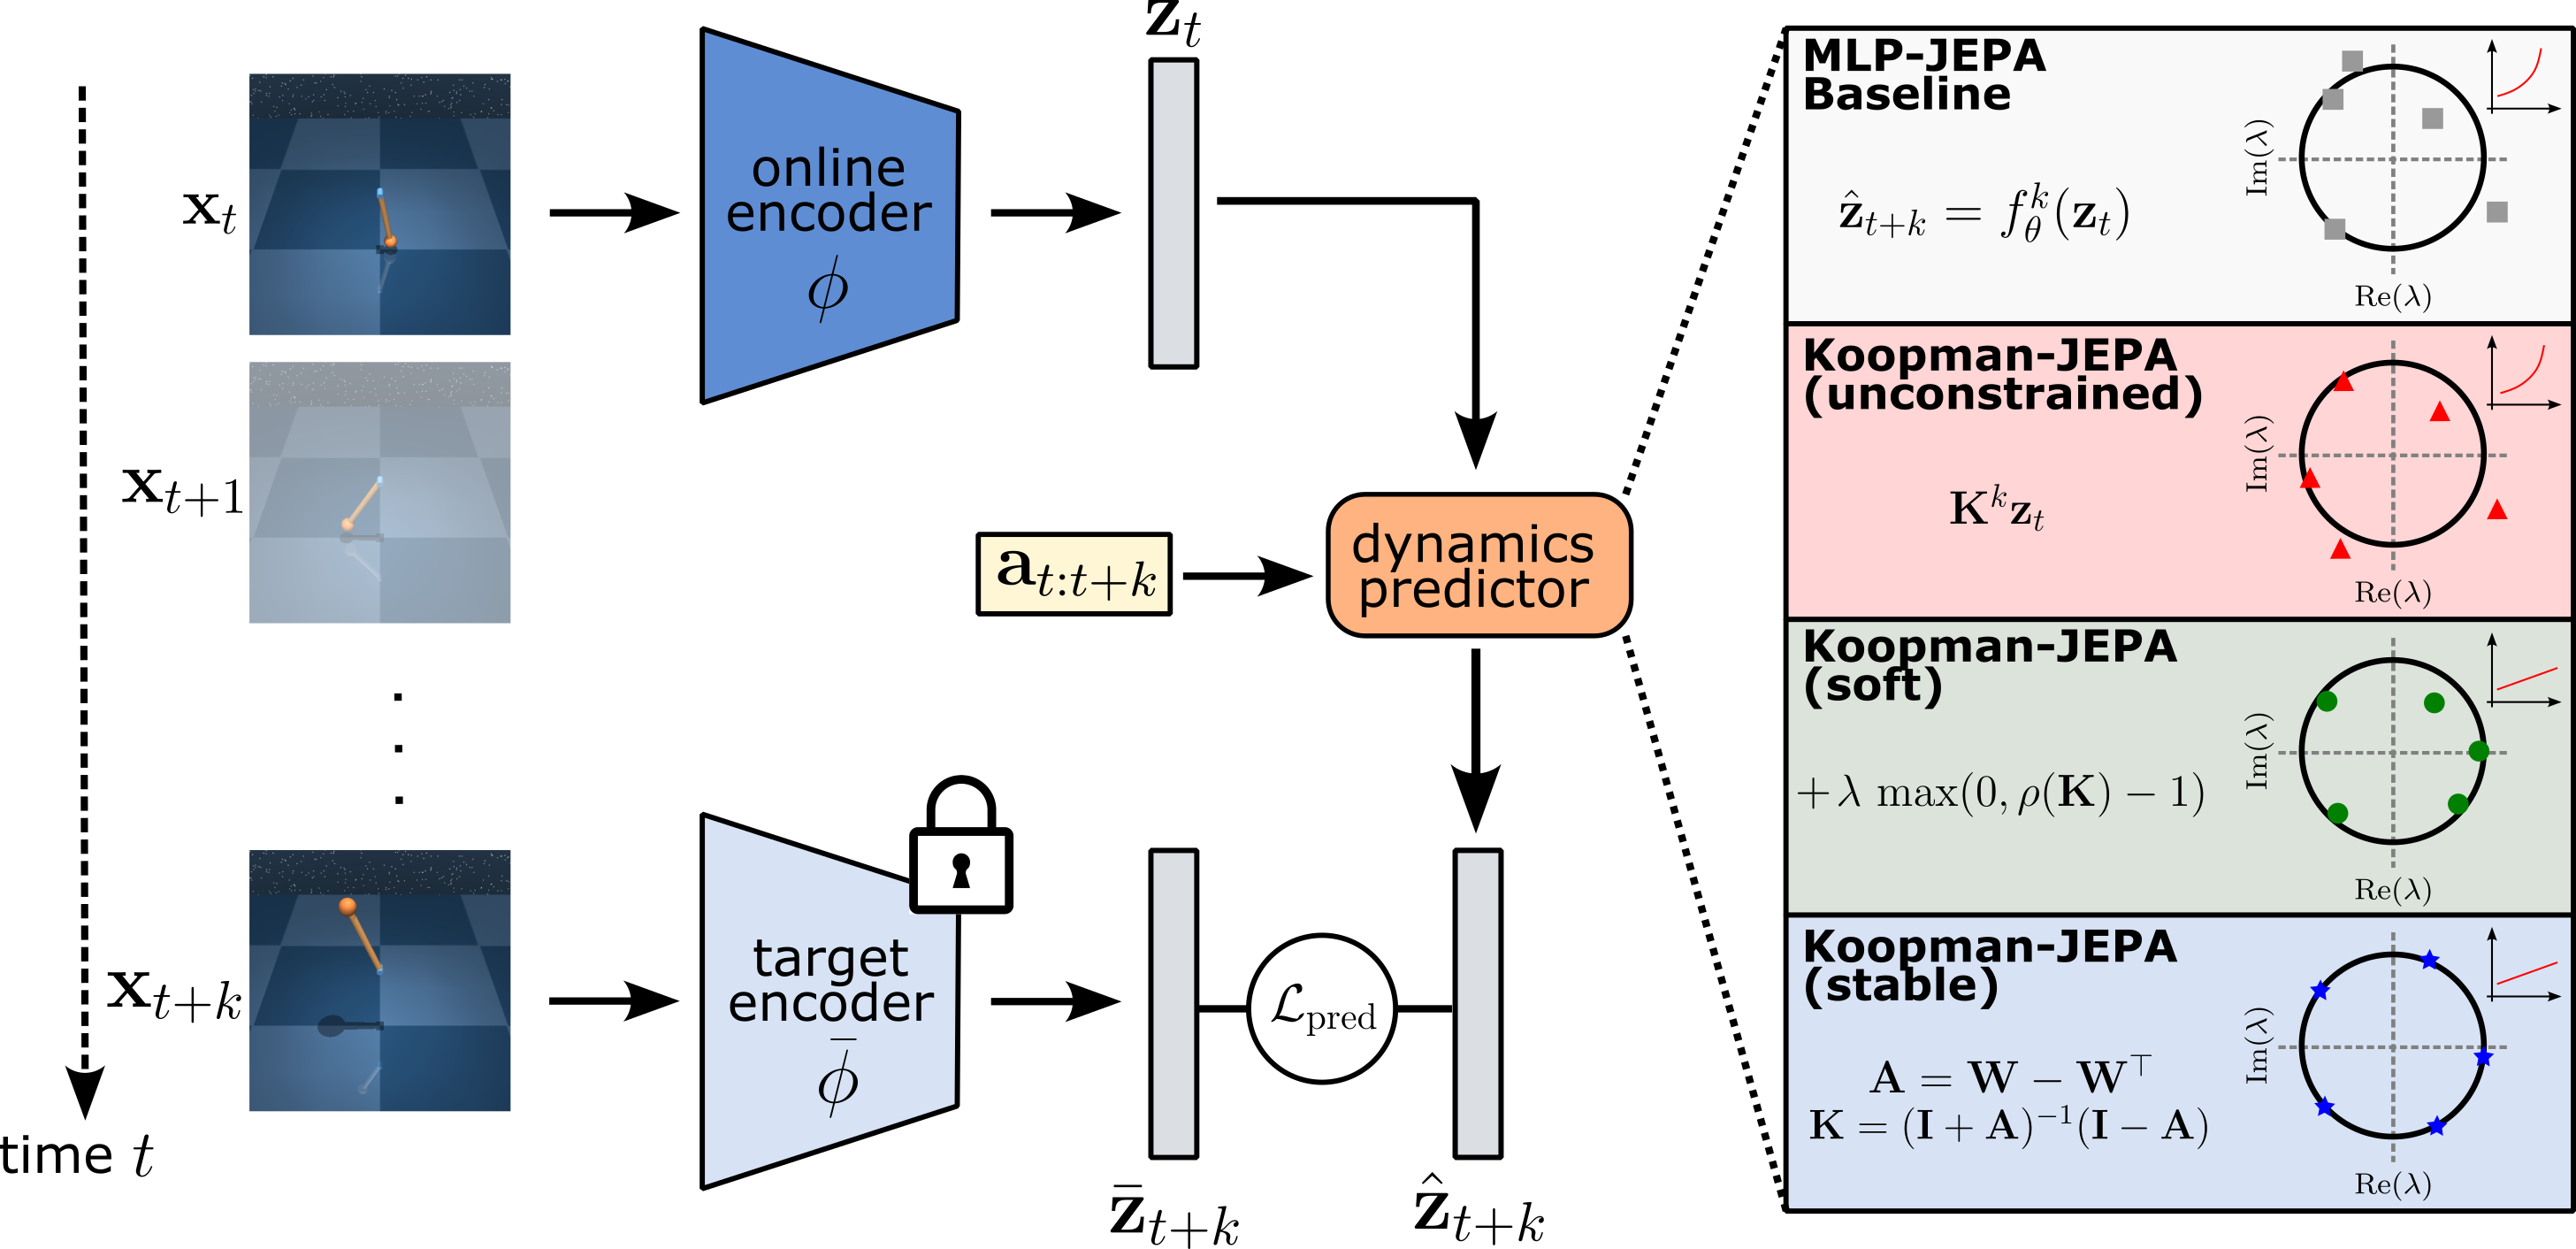
\includegraphics[width=0.76\textwidth]{paper_figures/koopman.png}
    \caption{The four dynamics modules differ only in how the spectrum of the
    transition operator is constrained. \textit{(Left)} An online encoder $\phi$
    maps the observation $\x_t$ to a latent $\z_t$, a dynamics module predicts
    future latents from an action sequence, and the prediction loss compares
    them against targets from an EMA-updated target encoder $\bar\phi$. No
    pixels are decoded during training. \textit{(Right)} The four modules. The
    MLP baseline has no transition matrix and so no spectrum, and the panel
    marks unbounded local amplification instead. Koopman~(Unconstrained) places
    no constraint on the eigenvalues of $\K$, Koopman~(Soft) penalizes a
    spectral radius above one, and Koopman~(Stable) forces every eigenvalue onto
    the unit circle through a Cayley transform. The inset sketches the error
    growth each implies.}
    \label{fig:architecture}
\end{figure*}

\subsection{Four Dynamics Modules, One Encoder and One Objective}
\label{sec:variants}
% [orig 4 p1, p2] DONE, verbatim except that the two forward references now
% point at appendices B and C, where the derivations live.
All four models share the same encoder and JEPA training scheme~\citep{LeCun2022,Assran2023,Bardes2024}. The dynamics module is the only component that differs, and no pixels are decoded during training. An online encoder $\phi_\theta: \mathcal{X} \to \mathbb{R}^D$ maps each $128{\times}128$ RGB frame $\x_t$ to a latent vector $\z_t = \phi_\theta(\x_t)$ ($D{=}256$, selected by the tuning protocol of Appendix~\ref{app:impl}). A target encoder $\bar\phi$, parameterized identically to $\phi_\theta$, is updated as an exponential moving average (EMA) of the online weights~\citep{Grill2020} to produce stable prediction targets $\bar{\z}_{t+k} = \bar\phi(\x_{t+k})$. The dynamics module $f_\theta$ produces the $k$-step latent prediction $\hat{\z}_{t+k} = f_\theta^k(\z_t, \mathbf{a}_{t:t+k})$, conditioned on the executed action sequence. Figure~\ref{fig:architecture} shows the resulting architecture and the four variants.

For $f_\theta$ we compare four choices that separate nonlinearity, linearity, and spectral constraint. The \emph{MLP-JEPA baseline} uses a three-layer residual network, the standard nonlinear choice, subject to the exponential compounding of Equation~\ref{eq:compound}. The three \emph{Koopman} variants replace it with a single linear matrix $\K$. When actions are available the state evolves as $\z_{t+1} = \K\z_t + \B\mathbf{a}_t$, where $\B \in \mathbb{R}^{D \times m}$ is an unconstrained linear layer that maps $m$-dimensional actions into the latent space. The variants differ only in how the eigenvalues of $\K$ are constrained: \emph{Koopman~(Unconstrained)} optimizes $\K$ freely, \emph{Koopman~(Soft)} penalizes any spectral radius in excess of one (Appendix~\ref{app:soft}), and \emph{Koopman~(Stable)} enforces $|\lambda_i(\K)| = 1$ exactly through a Cayley parameterization (Appendix~\ref{app:dmd}). Initialization details, including the DMD warm-start used by the Stable variant, are given in Appendix~\ref{app:dmd}.

% [orig, training objective] DONE. Compressed from six sentences to four.
% "additionally" dropped as a banned filler word, and the decoder pointer moved
% from the deleted visual-MSE appendix to Section 5.2, which is where the one
% surviving decoder measurement is reported.
The prediction loss $\mathcal{L}_\text{pred}$ is the cosine distance between $\hat{\z}_{t+k}$ and $\bar{\z}_{t+k}$, averaged over all horizons up to $H$ (with $H{=}6$ for our training sequences of length 8). To prevent representational collapse, the online representations are regularized with VICReg~\citep{Bardes2022}. Its variance term $\mathcal{L}_\text{var}$ keeps each latent dimension informative and its covariance term $\mathcal{L}_\text{cov}$ decorrelates dimensions. The total base loss is
\begin{equation}
    \mathcal{L}_\text{base} = \lambda_p\,\mathcal{L}_\text{pred} + \lambda_v\bigl(\mathcal{L}_\text{var} + \lambda_c\,\mathcal{L}_\text{cov}\bigr).
    \label{eq:base_loss}
\end{equation}
The prediction weight $\lambda_p$ is held at zero for a short warm-up period so the encoder can establish a spatial representation under VICReg alone, and the warm-up length and the weights $\lambda_p$, $\lambda_v$, $\lambda_c$ are selected per method by the protocol of Appendix~\ref{app:impl} (Table~\ref{tab:hyperparams}). Training proceeds in two phases: the encoder and dynamics module are first optimized jointly under this objective, then both are frozen and a convolutional decoder is trained separately for visualization, which plays no role in the dynamics training signal or in any reported metric.

\subsection{Environments, Protocol and Tuning}
\label{sec:protocol}
% [orig, results preamble] DONE, verbatim. The three paragraphs that set up the
% comparison move here from the old Results section, where they preceded the
% first table.
We evaluate the three Koopman variants against the nonlinear MLP-JEPA baseline on the pendulum- and cartpole-swingup tasks from the DeepMind Control Suite~\citep{Tassa2018}. To test visual robustness, we extend the evaluation to three levels of distraction complexity (\textit{easy}, \textit{medium}, \textit{hard}) using the Distracting Control Suite~\citep{Stone2021}, which combines dynamic natural-scene background videos with camera-pose and color perturbations of increasing magnitude (Figure~\ref{fig:environments}). All final results are computed on a held-out test set, disjoint from both training and model selection, averaged over 10 random seeds, and reported as means with 95\% bootstrap confidence intervals.

The MLP-JEPA baseline shares the encoder architecture, training objective, and data with the Koopman variants, and its remaining (optimization and loss) hyperparameters are tuned independently by the same held-out selection protocol (Appendix~\ref{app:impl}), so that the latent dynamics module is the only structural difference across the comparison and the baseline is not disadvantaged by shared hyperparameters. This MLP-on-JEPA design is also the standard choice in the JEPA literature~\citep{Bardes2024,zhou2025dinowmworldmodelspretrained}. We do not compare against world models with different representation objectives (e.g., Dreamer~\citep{Hafner2025}, TD-MPC2~\citep{Hansen2023}), since that would confound the representation objective with the dynamics module. The MLP dynamics module carries roughly three times more parameters than the linear Koopman dynamics ($\approx\!198$k vs.\ $\approx\!66$k), so the Koopman variants' advantage is not attributable to greater capacity.


\subsection{Measurements and Controls}
\label{sec:measurements}
% [draft 4.4 + orig] DONE. The draft's 699 words cut to about 440. The probe
% paragraph merges the approved "Evaluation Metrics" text with the approved
% "Probe Choice" limitation, which is why that limitation is not in Section 7.
% Every definition puts the description before the name, per the guide, and
% this is the only site where the five terms are emphasized.
% MOVED: the Riccati paragraph to appendix D, which is also where the solver is
% named, since a package name does not belong in the main text.
Section~\ref{sec:bound_limits} argued that a bounded error curve is not by itself evidence of a learned model. This subsection defines the readouts and the controls that separate the two. All of them reuse the trained checkpoints unchanged, and the controls differ from the learned models only in the dynamics.

\paragraph{Probe state MSE.}
To check whether the learned latent states capture the underlying physical dynamics, we fit a \emph{probe}~\citep{alain2016understanding}, a two-layer MLP with 64 hidden units trained with the world-model weights frozen, mapping latent vectors to ground-truth physical coordinates. The two hidden layers absorb natural coordinate changes such as angle to $(\sin\theta, \cos\theta)$, which a linear probe would penalize independently of the quality of the representation, so the probe tests whether physical structure is recoverable from the latent rather than whether it is linearly aligned with it. Probe state MSE is the squared error between the true physical trajectory and the probe's prediction over a latent rollout, and probe $R^2$ measures the single-frame encoding, with $R^2 < 0$ signalling collapse. The metric is reported in raw coordinate units, which carry no intrinsic scale, so every table also carries the constant predictor defined below as a reference level.

\paragraph{A scale-invariant second readout.}
The probe is fitted on encoded observations and then applied to latents the model has iterated on its own, so it is used away from the distribution it was fitted on, and it responds to the length of the vector it receives as well as to its direction. We add a readout with neither property. Encoding a bank of held-out frames, matching each predicted latent to the nearest bank entry by cosine similarity, and reporting the squared error of the true physical state of the frame retrieved gives a score that reads direction only, never returns a state the environment did not visit, and requires no fitting. We call this \emph{retrieval}.

\paragraph{Trivial predictors.}
Three controls replace the dynamics with something that cannot have learned them, while keeping each model's own encoder and probe. Copying the current latent forward unchanged, $\hat{\z}_{t+k} = \z_t$, is the operator $\K = I$ and is non-expansive. We call it \emph{persistence}. Returning the mean physical state of the training set at every horizon is the constant predictor of Section~\ref{sec:bound_limits}. We call it \emph{mean state}, and whichever of the two is more accurate in a given cell is the \emph{trivial floor}, the level any useful model has to clear. A third control substitutes a frozen \emph{random orthogonal} matrix for $\K$, which satisfies the Cayley variant's spectral guarantee exactly while having learned nothing, and so separates the value of the constraint from the value of training under it. The first two depend on the encoder only through the probe, and vary by under one percent across the four, so we pool them per environment into one row each.

\paragraph{Spectral rescaling.}
Rescaling a learned operator to a target spectral radius, $\K \leftarrow (\rho_\text{target} / \rho(\K))\,\K$, and re-running the rollout with the encoder, the probe and the action matrix untouched varies the one quantity the theory identifies while holding the learned features fixed. We call this \emph{spectral rescaling}, and use $\rho_\text{target} \in \{0.9, 0.95, 1.0, 1.05, 1.1, 1.2\}$.

% =============================================================================
\section{Results}
\label{sec:exp}

\subsection{Measured the Standard Way, the Constraint Wins}
\label{sec:results}
\begin{table}[t]
\caption{Learned latent dynamics against trivial controls, clean backgrounds, at horizons $T{=}10$ / $T{=}20$. Probe state MSE ($\downarrow$), mean $\pm$ 95\% bootstrap-CI half-width ($B{=}10000$) over 10 seeds; $\dagger$ marks heavy-tailed cells whose across-seed standard deviation exceeds the mean, where the mean is set by one or two divergent seeds and the median is substantially lower; ($\boldsymbol{\nabla}$) is the relative error reduction vs.\ the MLP-JEPA baseline; $^{\ast}$ = worse than that baseline. \textbf{Bold} = best in the block, controls included. The two controls use each model's own encoder and probe and differ only in the dynamics, so they are pooled over all 40 checkpoints of the environment ($R^2$ is a property of the shared encoder and is therefore not repeated for them). On pendulum the probe target is $[\sin\theta, -\cos\theta, 0, 0]$, whose two live dimensions place chance level at $0.5$.}
\label{tab:combined}
\centering
\small
\begin{tabular}{@{} l l@{\hspace{0.6em}}l l@{\hspace{0.6em}}l l @{}}
\toprule
\textbf{Configuration} & \multicolumn{2}{l}{\textbf{Probe MSE $T{=}10\downarrow$ ($\boldsymbol{\nabla}$)}} & \multicolumn{2}{l}{\textbf{Probe MSE $T{=}20\downarrow$ ($\boldsymbol{\nabla}$)}} & \textbf{Probe $R^2 \uparrow$} \\
\midrule
\multicolumn{6}{c}{\textbf{Pendulum}} \\
\midrule
Koopman~(Stable)                   & $5.62 \pm 0.718$ & ($-$39\%) & $3.68 \pm 0.386$ & ($-$100\%) & $0.651 \pm 0.005$ \\
Koopman~(Soft)                     & $4.22 \pm 0.409$ & ($-$54\%) & $20.3 \pm 22.5{}^\dagger$ & ($-$100\%) & $0.664 \pm 0.004$ \\
Koopman~(Unconstrained)            & $131 \pm 74.7$ & ($+$1330\%)$^{\ast}$ & $8.6{\times}10^{5} \pm 6.7{\times}10^{5}{}^\dagger$ & ($+$13362\%)$^{\ast}$ & $0.663 \pm 0.005$ \\
MLP-JEPA baseline                  & $9.19 \pm 6.41{}^\dagger$ &  & $6354 \pm 8780{}^\dagger$ &  & $0.666 \pm 0.002$ \\
\midrule
\emph{Persistence} (copy $\z_t$)   & $5.44 \pm 0.076$ & ($-$41\%) & \boldmath $1.66 \pm 0.047$ & ($-$100\%) & -- \\
\emph{Mean-state} (dataset mean)   & \boldmath $3.52 \pm 0.000$ & ($-$62\%) & $2.51 \pm 0.000$ & ($-$100\%) & -- \\
\midrule
\multicolumn{6}{c}{\textbf{Cartpole}} \\
\midrule
Koopman~(Stable)                   & $0.843 \pm 0.324$ & ($-$69\%) & $24.7 \pm 20.3{}^\dagger$ & ($-$99\%) & $0.607 \pm 0.012$ \\
Koopman~(Soft)                     & $0.609 \pm 0.301$ & ($-$78\%) & $13.5 \pm 8.39{}^\dagger$ & ($-$99\%) & $0.452 \pm 0.056$ \\
Koopman~(Unconstrained)            & $1.42 \pm 0.776$ & ($-$48\%) & $399 \pm 152$ & ($-$79\%) & $0.500 \pm 0.034$ \\
MLP-JEPA baseline                  & $2.72 \pm 0.945$ &  & $1874 \pm 2305{}^\dagger$ &  & $0.620 \pm 0.025$ \\
\midrule
\emph{Persistence} (copy $\z_t$)   & $0.461 \pm 4.6{\times}10^{-3}$ & ($-$83\%) & $1.03 \pm 4.4{\times}10^{-3}$ & ($-$100\%) & -- \\
\emph{Mean-state} (dataset mean)   & \boldmath $0.405 \pm 0.000$ & ($-$85\%) & \boldmath $0.975 \pm 0.000$ & ($-$100\%) & -- \\
\bottomrule
\end{tabular}
\end{table}

% [orig 5.1 + new] DONE. The first paragraph keeps the approved paper's
% reading of the separation, in its own terms, on the seeded numbers. The
% second is new and is the point of the section.
Measured the way this literature measures, the constraint works. Table~\ref{tab:combined} reports probe state MSE at $T{=}10$ and $T{=}20$ on clean backgrounds at full data. At $T{=}20$ on pendulum the four dynamics modules span more than five orders of magnitude, from $3.68$ for Koopman~(Stable) to $8.6\times10^{5}$ for the unconstrained operator, with the MLP-JEPA baseline at $6.4\times10^{3}$. Cartpole separates the same way and a constrained operator again leads, Koopman~(Soft) at $13.5$ against $1.9\times10^{3}$ for the baseline. The spectra are consistent with the ordering: the unconstrained operator's eigenvalues drift outside the unit circle ($\rho(\K) = 1.43$), the soft variant settles just outside it ($1.04$), and the Cayley variant sits exactly on it by construction (Figure~\ref{fig:eigenvalues}). Linearity by itself is not what separates them, since the unconstrained linear operator diverges alongside the nonlinear baseline.

The control rows change the reading. One of the two trivial predictors is the most accurate entry in every block of the table. On pendulum at $T{=}20$ the best learned model reads $3.68$ against $1.66$ for copying the current latent forward. On cartpole it reads $13.5$ against $0.98$ for the dataset mean. Counting every environment, dynamics module and horizon at $T \ge 10$, a trivial predictor wins $24$ of $24$ cells, and $168$ of $168$ once all four backgrounds and all four data fractions are included (Appendix~\ref{app:full_results}). The learned models win only at the shortest horizon, and only on cartpole, where three of the four beat the floor by between $4$ and $15$ percent.

Section~\ref{sec:bound_limits} anticipated this. A predictor that cannot amplify its input has a flat error curve whether or not it has learned the dynamics, and both controls are of that kind. What Table~\ref{tab:combined} establishes is therefore not that the constraint helps, but that the probe ranks the constrained operators first while ranking two predictors that learned nothing ahead of all of them.

\subsection{The Advantage Evaporates under a Scale-Invariant Readout}
\label{sec:inversion}
\begin{table}[t]
\caption{The same rollouts under two readouts, clean backgrounds at full data, mean over 10 seeds. \emph{Probe} decodes the physical state from the rolled-out latent; \emph{retrieval} matches the latent to the nearest encoded held-out frame and scores that frame's true state (Section~\ref{sec:measurements}). The ratio is the factor by which the probe reads worse than retrieval on identical rollouts. \textbf{Bold} = best learned model in the block under that readout. Persistence is included as an internal check: it does not drift in norm, and the two readouts agree on it to within one percent.}
\label{tab:retrieval}
\centering
\small
\begin{tabular}{@{}lcccccc@{}}
\toprule
\textbf{Configuration} & \multicolumn{3}{c}{$T{=}10$} & \multicolumn{3}{c}{$T{=}20$} \\
 & \textbf{probe} & \textbf{retr.} & \textbf{ratio} & \textbf{probe} & \textbf{retr.} & \textbf{ratio} \\
\midrule
\multicolumn{7}{c}{\textbf{Pendulum}} \\
\midrule
Koopman~(Stable)         & $5.62$ & $6.93$ & $0.811$ & $\mathbf{3.68}$ & $\mathbf{4.05}$ & $0.908$ \\
Koopman~(Soft)           & $\mathbf{4.22}$ & $7.72$ & $0.546$ & $20.3$ & $4.72$ & $4.30$ \\
Koopman~(Unconstrained)  & $131$ & $7.19$ & $18.3$ & $8.6{\times}10^{5}$ & $5.61$ & $1.5{\times}10^{5}$ \\
MLP-JEPA baseline        & $9.19$ & $\mathbf{6.36}$ & $1.44$ & $6354$ & $4.90$ & $1297$ \\
\midrule
\emph{Persistence}             & $5.44$ & $10.5$ & $0.519$ & $1.66$ & $1.60$ & $1.04$ \\
\midrule
\multicolumn{7}{c}{\textbf{Cartpole}} \\
\midrule
Koopman~(Stable)         & $0.843$ & $0.569$ & $1.48$ & $24.7$ & $1.49$ & $16.6$ \\
Koopman~(Soft)           & $\mathbf{0.609}$ & $\mathbf{0.485}$ & $1.26$ & $\mathbf{13.5}$ & $\mathbf{1.12}$ & $12.1$ \\
Koopman~(Unconstrained)  & $1.42$ & $0.554$ & $2.57$ & $399$ & $1.54$ & $259$ \\
MLP-JEPA baseline        & $2.72$ & $0.634$ & $4.30$ & $1874$ & $1.68$ & $1117$ \\
\midrule
\emph{Persistence}             & $0.461$ & $0.565$ & $0.817$ & $1.03$ & $1.13$ & $0.914$ \\
\bottomrule
\end{tabular}
\end{table}

% [draft 5.2, rewritten on the seeded numbers] DONE. Two claims from the draft
% are gone because the data does not support them. The draft said the ranking
% inverts; it does not, the order is identical under both readouts on both
% environments and what collapses is the spread. The draft also said the two
% readouts agree on persistence to within one percent; the measured gap is four
% percent on pendulum and nine on cartpole, so the sentence says "a few
% percent". The decoder sentence is dropped: visual MSE was only ever measured
% on the superseded pass and is not in the ledger.
Table~\ref{tab:retrieval} scores the same rollouts twice, once with the probe and once with the scale-invariant readout of Section~\ref{sec:measurements}. Under the probe at $T{=}20$ on pendulum the four methods span a factor of $2.3\times10^{5}$, from $3.68$ for Koopman~(Stable) to $8.6\times10^{5}$ for the unconstrained operator. Under retrieval the same rollouts span a factor of $1.38$, from $4.05$ to $5.61$. On cartpole a spread of $139$ becomes $1.50$. Nothing about the rollouts changed between the two columns, only what is read off them.

The ordering does not change. Under both readouts, on both environments, the four methods rank in the same order, so this is a collapse rather than a reshuffle: a separation of five orders of magnitude becomes a separation of forty percent. Nor does the scale-invariant readout reveal a hidden winner. No learned model is meaningfully better than persistence under it, the closest being the soft variant on cartpole at $1.12$ against $1.13$.

The ratio column localizes the disagreement. It is near one for persistence, which by construction neither grows nor shrinks the latent, so the two readouts agree on it to within a few percent. It is $0.91$ for Koopman~(Stable), whose operator preserves norm by construction, rises to $4.3$ for the soft variant, whose spectral radius sits slightly above one, and reaches $1.3\times10^{3}$ for the baseline and $1.5\times10^{5}$ for the unconstrained operator. That is the ordering of how far each operator lets the latent norm travel, which is the quantity Section~\ref{sec:variants} noted the training objective does not constrain.

That last step is an inference from two readouts, and it can be checked directly on the operators. Rolling encoded held-out frames forward and recording the median of $\|\K^k\z\| / \|\z\|$ gives, on pendulum at $T{=}20$, exactly $1.000$ for Koopman~(Stable), $4.2$ for the soft variant, $6.9\times10^{2}$ for the baseline and $6.0\times10^{3}$ for the unconstrained operator, and the ordering matches the ratio column (Appendix~\ref{app:drift}). Cartpole is a weaker test of the same claim. Every operator there stays within a factor of ten at $T{=}20$, and at that scale the growth ordering no longer reproduces the ratio ordering, as one should expect once the drift is small enough for other differences to matter.


\subsection{The Metric Measures the Constraint}
\label{sec:spectrum}
\begin{figure}[t]
    \centering
    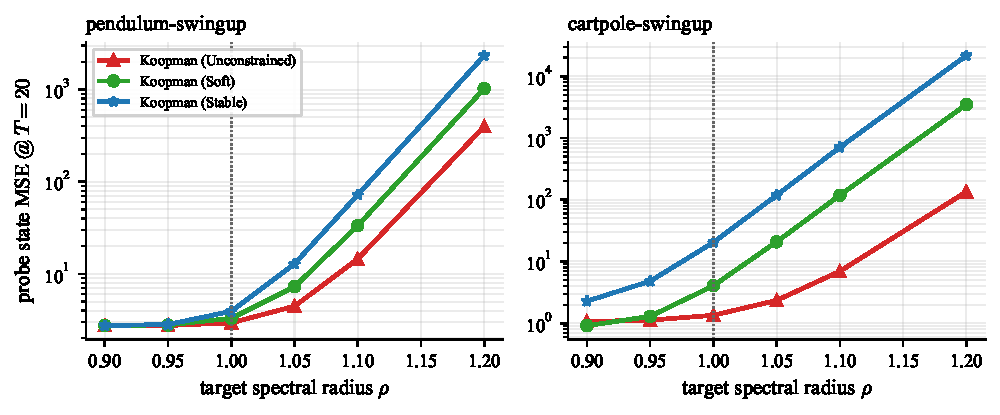
\includegraphics[width=\linewidth]{paper_figures/fig_rho_sweep.pdf}
    \caption{Probe error is governed by the spectral radius, and the response
    is monotone in all six curves. Each trained operator is rescaled to a target
    radius $\rho$ and the rollout is run again with the encoder, the probe and the
    action matrix untouched, so the only quantity that changes along a curve is
    the spectrum. \textbf{Left:} pendulum-swingup. \textbf{Right:}
    cartpole-swingup. Probe state MSE at $T{=}20$, mean over 10 seeds, log
    scale. The dotted line marks $\rho = 1$, the value the Cayley
    parameterization enforces. The lowest error on every curve is at
    $\rho = 0.9$. Values are comparable within a curve and not against
    Table~\ref{tab:combined}, which evaluates more episodes.}
    \label{fig:rho_sweep}
\end{figure}
% [new 5.3] DONE. The rho=1.0 point is not the Table 1 value for the same
% operator, because the sweep evaluates 20 episodes and the Table 1 rows
% evaluate 50. Every comparison here therefore stays inside one curve, and the
% caption says so.
Rescaling a trained operator to a target spectral radius and re-running the rollout moves the probe error monotonically, in all six curves of Figure~\ref{fig:rho_sweep}. On pendulum the Cayley operator rescaled to $\rho = 0.9$ reads $2.75$ at $T{=}20$, and the same operator at $\rho = 1.2$ reads $2.3\times10^{3}$, a factor of $850$ from a change that touches nothing but the spectrum. The encoder, the probe, the action matrix and the learned features are identical along each curve.

This is the intervention that the four-way comparison cannot perform. Comparing architectures varies the spectrum together with everything else that differs between them, whereas rescaling varies the spectrum alone, and the response is what Equation~\ref{eq:linear_bound} implies. Error growth tracks $\rho^k$. The theory is not what fails here. Every curve rises where the bound says it should.

The consequence is the point of this paper. The probe reads a latent by mapping it to physical coordinates, and it was fitted at the scale of encoded observations, so it charges a rollout for letting its norm run away. The bound limits exactly how far a rollout's norm can run away. Probe error and the quantity the bound constrains are therefore two measurements of the same thing, and an operator that satisfies the bound is guaranteed a flat probe curve whether or not it has learned the dynamics. The agreement between Table~\ref{tab:combined} and Equation~\ref{eq:linear_bound} that the study was designed to test is not a confirmation. It is one quantity measured twice. A bounded error curve under a norm-sensitive readout is a property of the constraint, not evidence of a learned model.

Two further readings follow from the figure. Contraction beats norm preservation, since the lowest error on all six curves is at $\rho = 0.9$ rather than at the $\rho = 1$ the Cayley parameterization enforces, so the architecture fixes the spectrum at a value the data does not prefer. And at a common $\rho$ the three operators differ far less than any one of them differs across $\rho$, which is another way of saying that the four-way comparison measured mostly the spectral radius.

\subsection{A Scale-Aware Loss Removes the Gap}
\label{sec:loss}
\begin{table}[t]
\caption{Does a scale-aware loss close the gap? Pendulum, clean backgrounds at full data, mean over 5 seeds. Both sides are measured in the same evaluation pass on the same held-out episodes, and differ in the prediction loss and nothing else. \emph{Ratio} is probe error divided by retrieval error on the same rollouts, so a value near one means the two readouts agree and the latent is not drifting in norm.}
\label{tab:l2_ablation}
\centering
\small
\begin{tabular}{@{}llcccccc@{}}
\toprule
\textbf{Configuration} & $T$ & \multicolumn{3}{c}{\textbf{cosine (paper)}} & \multicolumn{3}{c}{$\boldsymbol{\ell_2}$} \\
 & & probe & retr. & ratio & probe & retr. & ratio \\
\midrule
MLP-JEPA baseline & 10 & $338$ & $5.40$ & $62.6$ & $5.48$ & $7.04$ & $0.780$ \\
MLP-JEPA baseline & 20 & $1.0{\times}10^{7}$ & $3.89$ & $2.6{\times}10^{6}$ & $9.89$ & $4.25$ & $2.33$ \\
Koopman~(Unconstrained) & 10 & $81.3$ & $7.94$ & $10.2$ & $3.76$ & $5.93$ & $0.633$ \\
Koopman~(Unconstrained) & 20 & $2.3{\times}10^{5}$ & $4.24$ & $5.3{\times}10^{4}$ & $3.21$ & $5.88$ & $0.546$ \\
Koopman~(Stable) & 10 & $4.84$ & $7.68$ & $0.631$ & $5.99$ & $7.30$ & $0.821$ \\
Koopman~(Stable) & 20 & $3.62$ & $4.04$ & $0.895$ & $6.28$ & $4.50$ & $1.40$ \\
\bottomrule
\end{tabular}
\end{table}

% [new 5.4] DONE. Both arms are trained for this ablation, so the cosine
% column is not the Table 1 column: it is fifteen fresh runs on pendulum at
% clean backgrounds and full data. Saying so matters, because the alternative
% reading is that the comparison mixes the ablation against the main study.
Section~\ref{sec:inversion} attributes the gap between the two readouts to a training objective that does not constrain latent norm. If that is right, an objective that does constrain it should close the gap. Table~\ref{tab:l2_ablation} reports the test. Two arms of five seeds each are trained on pendulum with clean backgrounds and full data, differing only in the prediction loss, and both are evaluated on the same held-out episodes, so the dataset-mean control reads $2.51$ at $T{=}20$ for both.

The gap closes. Under the cosine objective the probe reads $2.6\times10^{6}$ times worse than retrieval for the MLP-JEPA baseline at $T{=}20$, and $5.3\times10^{4}$ times worse for the unconstrained operator. Replacing the cosine distance with an $\ell_2$ prediction loss brings those ratios to $2.33$ and $0.55$. The Cayley operator is the control here rather than the test: its ratio is already near one because the operator preserves norm by construction, and it stays near one under both objectives, $0.895$ against $1.40$. Four orders of magnitude of disagreement between two readouts are a property of the loss, and they can be removed by changing it.

Removing them does not produce a better model. Under the $\ell_2$ objective a trivial predictor is still more accurate than every learned model in all six cells, by $9.89$ against $1.65$ for the baseline at $T{=}20$ and $3.21$ against $1.71$ for the unconstrained operator. The recommendation this supports, which Section~\ref{sec:checklist} states, is about what the metric measures rather than about how well the models do.

\subsection{The Benchmark Degenerates, and the Control Claim Does Not Transfer}
\label{sec:degeneracy}
\begin{figure}[t]
    \centering
    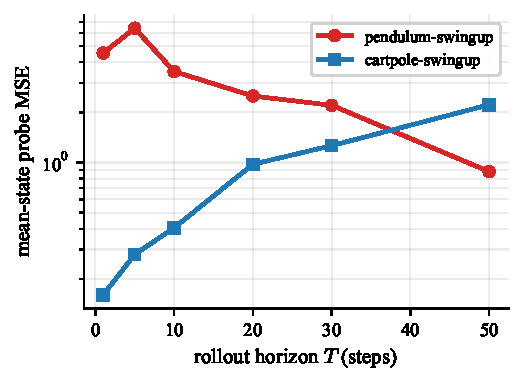
\includegraphics[width=0.48\linewidth]{paper_figures/fig_degeneracy.pdf}
    \caption{The pendulum benchmark stops discriminating at long horizon and
    cartpole does not. Error of the dataset-mean predictor against rollout
    horizon, log scale. A constant predictor cannot improve as the horizon
    grows unless the states it is asked to predict are themselves becoming more
    predictable, so the falling pendulum curve is evidence that they are. The
    predictor uses no model, so each curve is a property of the evaluation data
    rather than of any method, and is pooled over all checkpoints of the
    environment.}
    \label{fig:degeneracy}
\end{figure}
% [draft, compressed] DONE. The second paragraph is what remains of the
% approved paper's control section, which was a full section and is now a
% paragraph plus appendix D. It keeps the algebraic claim intact and reports
% what it buys.
A predictor that ignores its input cannot become more accurate as the horizon grows, unless the states it is asked to predict are themselves becoming more predictable. On pendulum they are. Figure~\ref{fig:degeneracy} plots the error of the dataset-mean predictor against horizon. It peaks at $6.41$ at $T{=}5$ and falls to $0.881$ by $T{=}50$, a factor of seven. Under a random policy the pendulum settles toward hanging, so the long-horizon state becomes predictable in advance of any model, and the benchmark stops separating methods at exactly the horizons where the compounding argument is most interesting. Cartpole does not degenerate, rising from $0.160$ to $2.22$ across the same range. The curve costs one line to plot and says whether a long-horizon benchmark still discriminates.

The control claim does not transfer either. The Cayley parameterization rules out divergent modes by construction, which removes one documented obstacle to a finite-cost discrete-time LQR, and that algebra holds. What it buys empirically is nothing. Solving the Riccati equation with a method that reports failure, rather than iterating the recursion and reading a gain off whatever it reaches, the unconstrained operator admits no stabilizing solution on any of the ten seeds in either environment. The Cayley operator admits one on all ten, and the resulting closed loop has spectral radius $0.9999$, a contraction so slight that a disturbance takes roughly $8{,}600$ steps to halve, against rollouts of $50$. With every mode on the unit circle, stabilizability needs all $D{=}256$ modes to be controllable through a scalar input, and the conditioning in Appendix~\ref{app:lqr} shows how far that is from holding.

% =============================================================================
\section{What to Report Instead}
\label{sec:checklist}
% [draft 7, trimmed] DONE. Six items to five, the closed-loop one having moved
% to Section 5.5. Item 3 gains the loss ablation, which the draft could only
% recommend and Section 5.4 now demonstrates. Item 4's claim is narrowed: the
% draft said the heavy-tailed cells are exactly the operators whose latents
% drift, which holds on pendulum and not on cartpole, where the Cayley variant
% is flagged too. The item now says what is true.
Every failure in this paper was caught by a measurement that costs close to nothing to add. None of them is novel in kind. Control tasks have been standard in probing since \citet{Hewitt2019ControlTasks}, copying the last frame has been a standard control in video prediction for as long~\citep{Villegas2017MCnet,Villegas2019HighFidelity}, and interval estimates have been urged on reinforcement learning by \citet{Agarwal2021Precipice}. What we add is the demonstration that their absence is not a stylistic omission, but enough to turn a careful comparison into a measurement artifact.

\begin{enumerate}
\item \textbf{Run trivial predictors through the model's own readout.} Copying the current latent forward and returning the dataset-mean state cost one line each, require no training, and set the level that any claim of learned dynamics has to clear. Our models did not clear it (Section~\ref{sec:results}). Route them through the same encoder and probe as the model, or the comparison measures the readout instead of the dynamics.

\item \textbf{Plot the constant predictor against the horizon.} It cannot improve as the horizon grows unless the targets are collapsing, so a falling curve is evidence that the benchmark has stopped discriminating. Ours falls by a factor of seven from its peak on pendulum (Section~\ref{sec:degeneracy}).

\item \textbf{Pair a scale-sensitive readout with a scale-invariant one.} Where the two agree, the readout is not the story. Where they disagree, the gap localizes what the training objective failed to constrain, which was the whole result of Section~\ref{sec:inversion}. Better still, remove the mismatch at its source by training with a loss that sees the same geometry the metric does, which closes the gap (Section~\ref{sec:loss}).

\item \textbf{Report the tail, not only the center.} Heavy tails are often the artifact rather than noise around it. On pendulum, every cell of Table~\ref{tab:combined} whose across-seed standard deviation exceeds its mean belongs to an operator whose latents drift, and none belongs to the operator that preserves norm.

\item \textbf{Vary the mechanism directly when the model permits it.} Comparing architectures confounds the property of interest with everything else that differs between them. Rescaling a trained operator moves one quantity and holds the rest fixed, and it gave a cleaner answer about the spectrum than the four-way comparison the study was designed around (Section~\ref{sec:spectrum}).
\end{enumerate}

The first four apply to any evaluation that rolls a latent forward and reads it out, the fifth wherever the mechanism is exposed as a parameter. All five are implemented in the diagnostics released with the paper, and Appendix~\ref{app:provenance} records which file produced each number.

% =============================================================================
\section{Limitations}
\label{sec:limitations}
% [draft 8 p1] DONE. Two changes to the draft. "We think this reading
% strengthens the case" becomes a statement of what the evidence shows, per the
% guide. And the draft named which control wins where, "mean-state on pendulum,
% persistence on cartpole", which is wrong on the seeded numbers: mean state
% wins three of the four tabulated cells and persistence the fourth. The
% sentence no longer needs the split, so it does not make the claim.
\paragraph{An Alternative Reading of the Gap.}
We read the disagreement of Section~\ref{sec:inversion} as a measurement artifact, and the opposite reading deserves stating in its strongest form. Every fixed readout of a latent state is fitted at some scale, whether it is a probe, a decoder, a value head or a controller, and a latent that leaves that scale is unusable to all of them however well it points. On that view the probe is not misreporting anything. It records a real failure that a downstream consumer would also suffer, and retrieval is the lenient metric, because cosine matching discards exactly the information such a consumer would need.

That reading strengthens the case for reporting the controls rather than weakening it. It is a claim about the readout and not about the dynamics, so it leaves the trivial predictors where they were. On the probe, the very metric this reading defends, a trivial predictor is the most accurate entry in both environments at both tabulated horizons (Table~\ref{tab:combined}). Accepting the alternative reading therefore relocates the failure rather than repairing it, from a metric that misreads the models to a metric on which the models lose to copying their own input. And if latent scale is what matters downstream, then controlling it is the objective, which Section~\ref{sec:spectrum} does at no training cost and slightly better than the architecture does.

% [orig, Empirical Scope] DONE, verbatim, with two sentences added on the
% behaviour policy. The draft's version of that addition said the random policy
% was used "rather than the intended mixture with an expert", which describes
% how the data came about rather than what it means for the claim. What matters
% to a reader is that the policy is random and that this is what narrows the
% pendulum distribution, so the sentences say that and nothing else.
% CONSUMED: the approved "Probe Choice" limitation paragraph is not ported
% here. Its content, that a two-layer probe absorbs coordinate changes a linear
% probe would penalize, belongs with the definition of the probe and lands in
% Section 4.3 at step 3.3.
\paragraph{Empirical Scope.}
Our environments are chosen for the falsifiability of the central spectral claim, not for visual complexity. The classical control benchmarks give us the ground-truth transparency to validate the bound of Equation~\ref{eq:linear_bound} against known physics. Scaling to richer environments (e.g., humanoid or wheeled-legged robots) raises distinct challenges. In contact-rich physics, the continuous dynamics are punctuated by discrete impacts, and a single global linear operator may struggle to capture these piecewise-linear regime shifts. A potential solution is to scale the latent dimension beyond $D{=}256$ and adopt a switching-Koopman architecture, where a learned gating mechanism selects from a library of specialized operators $\{\K_1, \dots, \K_M\}$ depending on the active interaction regime. Within these two environments the episodes are collected under a uniformly random policy, which is what narrows the pendulum state distribution at long horizons (Section~\ref{sec:degeneracy}). A mixture with an expert policy would broaden it, and would raise the level a trivial predictor has to clear.
% [draft 8 p3] DONE, trimmed. The draft's closing sentence said retrieval was
% computed only for the clean, full-data cell, so the later sections stayed
% probe-only. That caveat is gone because retrieval now exists in all 560
% cells, which is what Appendix E reports.
\paragraph{What Retrieval Cannot Do.}
Retrieval has biases of its own. It cannot resolve a prediction more finely than the spacing of the frames in its bank, so it compresses differences between models that are all accurate, and it flatters any model whose errors stay on the data manifold. It is a differently biased readout rather than a correct one, and the argument of Section~\ref{sec:inversion} rests on the disagreement between the two, not on either being authoritative.

% [new] DONE.
\paragraph{One Instance of a General Mechanism.}
The confound needs three ingredients: a prediction loss that is invariant to latent scale, a readout fitted at a fixed scale, and an autoregressive rollout that leaves the scale free to drift. All three are ordinary in the JEPA world-model line, and Section~\ref{sec:loss} identifies the loss as the lever, since changing that alone removes the gap. We have measured no pipeline but our own. Whether the same gap opens elsewhere is a question this design can pose and not answer, and the cheapest way to find out is the pairing of readouts in Section~\ref{sec:checklist}, which needs one extra evaluation pass and no retraining.

% =============================================================================
\section{Conclusions}
\label{sec:conclusion}
% [new] DONE. No future-work subsection: the approved paper had one and it
% proposed extensions to a method this paper no longer recommends.
A bounded error curve under a norm-sensitive readout is a property of the constraint, not evidence of a learned model. That is the finding, and it comes out of a study built to test something else.

The theory is intact. Rescaling a trained operator moves probe error monotonically in all six curves we measure, as the error bound implies, and the Cayley parameterization holds latent norm at $1.000$ across every horizon, as orthogonality requires. What does not follow is the step from that guarantee to better prediction. Under a readout that ignores latent scale, the five orders of magnitude separating the four dynamics modules become a factor of $1.38$, and under either readout two predictors that learned nothing are more accurate than all of them.

The constraint is not useless. It controls latent norm, which is worth something once the measurement is right, and Section~\ref{sec:spectrum} shows that rescaling a trained operator controls it more cheaply and at a better spectral radius than the architecture does. What the constraint does not do is the thing the probe appeared to say it did. Separating the two took two trivial predictors and a second readout.

\subsubsection*{Broader Impact Statement}
% [orig] verbatim.

\subsubsection*{Acknowledgments}
Anonymized for double blind review.

\bibliography{main}
\bibliographystyle{tmlr}

\appendix

% =============================================================================
\section{Implementation Details}
\label{app:impl}
% [orig app] DONE. Verbatim except that the temporal-masking subsection is
% deleted, the Section 4.1 pointer is renamed, and the opening sentence says
% which claim the appendix supports.
This appendix supports the claim of Section~\ref{sec:protocol} that the dynamics module is the only component that varies across the four models.

The encoder architecture is selected by the tuning protocol below. The selected configuration, shared by all four methods, consists of three stride-2 convolutional blocks (channel widths 16, 32, 64) with Group Normalization and GELU activations, mapping $128{\times}128$ RGB inputs to a $16{\times}16$ spatial feature map, followed by a two-layer MLP (bottleneck dimension 256) with Layer Normalization, producing a $D{=}256$ dimensional latent vector.

\paragraph{Hyperparameter selection.} We select hyperparameters in two stages, both under a protocol fixed in advance of the final runs that scores every configuration by 1-step probe state MSE on a held-out validation split, disjoint from both the training and the test episodes. This criterion is short-horizon and penalizes representational collapse, and it does not select for the long-horizon behavior we report, so long-horizon performance was not optimized during model selection.
\begin{description}
\item[Stage 1 (shared architecture).] We first search the encoder architecture, jointly with the optimization and loss hyperparameters (Table~\ref{tab:search_space}), on the MLP-JEPA baseline alone (32 random trials per environment), and fix the winning encoder as the shared backbone for all four methods. Fixing a single architecture is what makes the comparison controlled: the dynamics module is then the only component that varies, so a performance difference can be attributed to it rather than to encoder capacity. We deliberately tune this architecture on the baseline, the most flexible model, so that the shared backbone is the one best suited to the strongest competitor and cannot be suspected of being tailored to favor the linear Koopman operators.
\item[Stage 2 (per-method optimization).] With the encoder frozen, we then tune the optimization and loss hyperparameters of each method independently (Table~\ref{tab:search_space}), again 32 trials each. The four dynamics modules induce very different optimization landscapes, for instance the spectral radius penalty and the warm-up schedule apply to only some variants, so a single shared setting would arbitrarily disadvantage some methods. Each method is therefore evaluated at the best configuration found within its own 32-trial budget.
\end{description}
Each selected configuration is finally trained for 2000 epochs and evaluated over 10 seeds. The selected per-method values are listed in Table~\ref{tab:hyperparams}.

\begin{table}[ht]
\caption{Random-search grid for hyperparameter selection (Appendix~\ref{app:impl}). Architecture is searched in Stage~1 on the MLP-JEPA baseline only, to fix the shared encoder; the optimization and loss hyperparameters are searched independently per method (32 trials each). $\lambda_s$ (the spectral-radius penalty) is active only for Koopman~(Soft).}
\label{tab:search_space}
\centering
\small
\begin{tabular}{@{}ll@{}}
\toprule
\textbf{Hyperparameter} & \textbf{Search grid} \\
\midrule
\multicolumn{2}{c}{\textbf{Architecture (Stage 1)}} \\
\midrule
Latent dimension $D$          & $\{32,\ 64,\ 128,\ 256\}$ \\
Encoder base channels         & $\{16,\ 32,\ 64\}$ \\
Encoder depth                 & $\{3,\ 4,\ 5\}$ \\
MLP bottleneck width          & $\{256,\ 512,\ 1024\}$ \\
\midrule
\multicolumn{2}{c}{\textbf{Optimization \& loss (Stage 2)}} \\
\midrule
Learning rate                 & $\{3{\times}10^{-5},\ 10^{-4},\ 3{\times}10^{-4},\ 10^{-3}\}$ \\
Batch size                    & $\{16,\ 32,\ 64\}$ \\
EMA rate $\tau$               & $\{0.99,\ 0.995,\ 0.999\}$ \\
Warm-up epochs                & $\{0,\ 50,\ 100\}$ \\
Prediction weight $\lambda_p$ & $\{1,\ 5,\ 10\}$ \\
VICReg weight $\lambda_v$     & $\{0.5,\ 1,\ 2\}$ \\
Covariance weight $\lambda_c$ & $\{0.01,\ 0.04,\ 0.1\}$ \\
Spectral penalty $\lambda_s$  & $\{0.01,\ 0.05,\ 0.2,\ 0.5\}$ \\
\bottomrule
\end{tabular}
\end{table}


\begin{table}[ht]
\caption{Selected per-method hyperparameters (search grids in Table~\ref{tab:search_space}). The encoder architecture ($D{=}256$, base channels 16, depth 3, MLP bottleneck 256) is shared across all four methods (chosen by the Stage-1 baseline search); the optimization and loss hyperparameters below are selected independently per method by 1-step held-out probe state MSE. Fixed across all runs: sequence length 8, frame skip 5, $128{\times}128$ input, 200 training episodes, AdamW, Phase-1/Phase-2 epochs $2000/500$.}
\label{tab:hyperparams}
\centering
\small
\begin{tabular}{@{}llrrrrrrrr@{}}
\toprule
\textbf{Env} & \textbf{Method} & \textbf{LR} & \textbf{Batch} & \textbf{$\tau_{\rm EMA}$} & \textbf{Warmup} & \textbf{$\lambda_p$} & \textbf{$\lambda_v$} & \textbf{$\lambda_c$} & \textbf{$\lambda_s$} \\
\midrule
Pendulum & Koopman (Stable) & 3e-05 & 64 & 0.999 & 100 & 5 & 2 & 0.01 & 0.05 \\
Pendulum & Koopman (Soft) & 0.001 & 64 & 0.99 & 100 & 5 & 0.5 & 0.01 & 0.5 \\
Pendulum & Koopman (Unconstrained) & 3e-05 & 32 & 0.999 & 0 & 5 & 0.5 & 0.04 & 0.05 \\
Pendulum & MLP-JEPA baseline & 3e-05 & 64 & 0.99 & 0 & 10 & 0.5 & 0.1 & 0.05 \\
\midrule
Cartpole & Koopman (Stable) & 0.0001 & 64 & 0.995 & 0 & 10 & 1 & 0.01 & 0.05 \\
Cartpole & Koopman (Soft) & 0.0001 & 16 & 0.995 & 50 & 5 & 0.5 & 0.1 & 0.05 \\
Cartpole & Koopman (Unconstrained) & 0.0001 & 64 & 0.99 & 100 & 5 & 0.5 & 0.04 & 0.05 \\
Cartpole & MLP-JEPA baseline & 0.0001 & 64 & 0.99 & 50 & 10 & 0.5 & 0.04 & 0.05 \\
\bottomrule
\end{tabular}
\end{table}


\subsection{Data Collection}
Both environments use the same protocol. Episodes are collected under a uniformly random policy, and the executed action sequence is recorded and supplied to the model at training and evaluation time. Random exploration covers a wider region of the state space than expert trajectories would and prevents overfitting to a narrow behavioral distribution. Because the environments are deterministic and the actions are observed, the future trajectory is fully determined by the initial state, and long-horizon error reflects model error rather than environment stochasticity. The remaining ambiguity is in the initial condition, since the encoder receives a single frame and cannot observe velocity. This sets a floor on achievable long-horizon accuracy that applies equally to all four dynamics modules.

\begin{figure}[t]
    \centering
    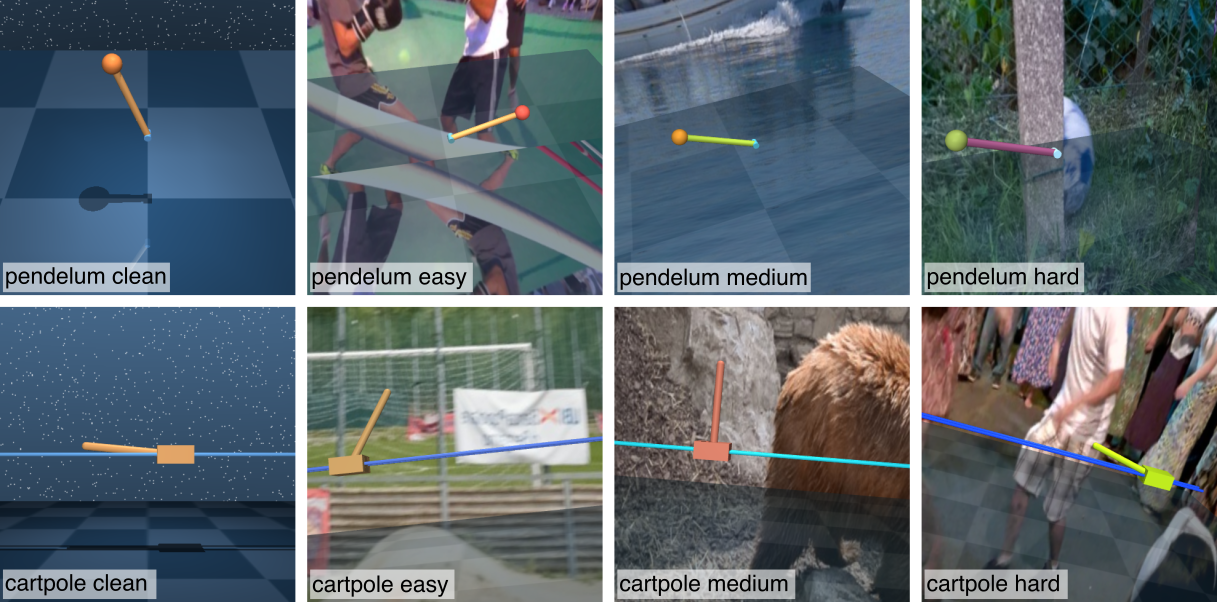
\includegraphics[width=0.64\linewidth]{paper_figures/environments_overview.png}
    \caption{Sample frames from the two evaluation environments across background conditions (left to right: clean, easy, medium, hard). \textbf{Top:} Pendulum-swingup. \textbf{Bottom:} Cartpole-swingup. Both are action-conditioned and collected under a random policy.}
    \label{fig:environments}
\end{figure}

\subsection{Training Phases}
Training proceeds in two phases.
Phase~1 ($2000$ epochs) jointly trains the encoder and dynamics module using the JEPA objective (Section~\ref{sec:variants}). We retain the checkpoint with the lowest 1-step validation probe state MSE, which is the model carried into Phase~2 and evaluated.
The prediction weight $\lambda_p$ is held at zero for a per-method warm-up period (from 0 to 100 epochs, Table~\ref{tab:hyperparams}) to let the encoder establish a meaningful representation via VICReg alone, then raised to its selected value.
Phase~2 ($500$ epochs) freezes the encoder and dynamics, training only a convolutional decoder to map latent states back to pixels.
The decoder is used solely for visualization and does not influence the dynamics evaluation.

% =============================================================================
\section{The Soft Spectral Penalty}
\label{app:soft}
% [orig 4.2] DONE, verbatim. The two equations merge into one display, and the
% forward reference to the results now points at Section 5.1.
This appendix defines the constraint that the Koopman~(Soft) variant of Section~\ref{sec:variants} applies.

The soft variant penalizes eigenvalues of $\K$ outside the unit circle. The bound of Equation~\ref{eq:linear_bound} requires the spectral norm, $\|\K\|_2 \le 1$. We penalize the spectral radius $\rho(\K)$ instead, which governs the asymptotic growth rate $\rho(\K)^k$ but permits transient growth (see the footnote following Equation~\ref{eq:linear_bound}). Unlike the Cayley variant, the soft penalty leaves the model free to place eigenvalues strictly inside the unit circle and so to represent damping. A soft spectral norm penalty, which power iteration makes cheap~\citep{Miyato2018}, would keep that freedom under the stronger condition and is a natural extension of the variant studied here. The penalty is
\begin{equation}
    \mathcal{L}_\text{soft} = \max(0,\; \rho(\K) - 1),
    \qquad
    \mathcal{L} = \mathcal{L}_\text{base} + \lambda_s\,\mathcal{L}_\text{soft},
    \label{eq:soft_penalty}
\end{equation}
so it activates only when $\rho(\K) > 1$. The weight $\lambda_s$ is selected per method (Table~\ref{tab:hyperparams}). Section~\ref{sec:results} reports what this weaker constraint buys.

% =============================================================================
\section{The Cayley Parameterization and Its DMD Warm-Start}
\label{app:dmd}
% [orig 4.3 + orig app] DONE, verbatim, merged. The construction that used to
% sit in the methods section joins the derivations that used to sit in the
% appendix, so eq:cayley and its verification are in one place.
This appendix defines the constraint that the Koopman~(Stable) variant of Section~\ref{sec:variants} applies, and shows that it holds at every gradient step.

The soft penalty discourages $\K$ from amplifying inputs, but does not strictly prevent it. The Stable variant replaces the penalty with an architectural constraint that makes amplification impossible by construction. It forces $\K$ to be orthogonal ($\K^\top \K = I$), meaning it preserves vector norms exactly ($\|\K\z\| = \|\z\|$ for every $\z$). An orthogonal $\K$ acts as a strict rotation of the latent space, so a latent trajectory rolled out by repeated application of $\K$ can neither grow nor shrink, and divergence is structurally ruled out.

To make this constraint differentiable, we use the \emph{Cayley transform}~\citep{Erichson2019}. For an unconstrained learnable weight matrix $W \in \mathbb{R}^{D\times D}$, define the skew-symmetric matrix $A = W - W^\top$ (a matrix satisfying $A^\top = -A$), and set
\begin{equation}
  \K = (I + A)^{-1}(I - A).
  \label{eq:cayley}
\end{equation}
Numerically, we evaluate $\K$ by solving the linear system $(I+A)\K = (I-A)$ rather than computing the explicit inverse. For any $W$ the factors commute, and
\begin{equation}
    \K^\top\K
    = (I - A)^\top (I + A)^{-\top} (I + A)^{-1} (I - A)
    = (I + A) (I - A)^{-1} (I - A) (I + A)^{-1}
    = I,
\end{equation}
so $\K$ is orthogonal, and $|\lambda_i(\K)| = 1$ for every $W$ and therefore at every gradient step.

The constraint applies to the learned latent space, not to the physical state. The encoder applies a nonlinear lift rather than a change of basis, so the latent dynamics it induces need not share the spectrum of the physical system, and orthogonality of $\K$ does not assume the underlying system is lossless.

\paragraph{Initialization.}
The unconstrained and soft variants initialize $\K$ as the identity matrix perturbed by small Gaussian noise ($\sigma = 0.01$), which biases the starting eigenvalues toward the unit circle and keeps rollouts stable during early training. Since they optimize over all of $\mathbb{R}^{D\times D}$, no further care is needed. The Cayley variant is warm-started with Dynamic Mode Decomposition (DMD)~\citep{Schmid2010} instead, because training from a random $W$ was unstable in the early epochs, before the encoder has settled. DMD finds the single linear operator best matching a set of observed transition pairs, and so gives the optimizer a globally consistent starting point. The $n{=}3{,}000$ encoded transition pairs are sampled uniformly at random from the Phase 1 training buffer, and the DMD matrix is $\K_\text{DMD} = Z' Z^\dagger \in \mathbb{R}^{D\times D}$, where $Z^\dagger$ is the Moore-Penrose pseudoinverse.

\paragraph{Warm-starting the Cayley map.}
$\K_\text{DMD}$ is generally not orthogonal, so it cannot be used directly in a parameterization that requires a skew-symmetric input. We bridge the gap by inverting the Cayley map approximately and extracting its skew-symmetric component:
\begin{equation}
  A_0 = \mathrm{skew}\!\left((I + \K_\text{DMD})^{-1}(I - \K_\text{DMD})\right),
  \quad
  \mathrm{skew}(M) = \tfrac{1}{2}(M - M^\top).
\end{equation}
This initializes $W$ so that the resulting Cayley map produces an orthogonal $\K$ as close as possible to the data-driven DMD solution, which gradient optimization then refines.

% =============================================================================
\section{Why Closed-Form Control Does Not Follow}
\label{app:lqr}
% [orig app + orig 6 + draft 4.4 + new] DONE. The proposition moves here from
% the approved paper's Section 6, which is now the second paragraph of Section
% 5.5, so the statement and its proof are together for the first time.
This appendix checks the claim of Section~\ref{sec:degeneracy} that ruling out divergent modes does not deliver closed-form control.

\begin{proposition}[No divergent eigenmodes under orthogonal $\K$]
\label{prop:cayley-stab}
Let $\K \in \mathbb{R}^{D\times D}$ be the Cayley-parameterized transition matrix defined by Equation~\ref{eq:cayley} for any learnable weight matrix $W \in \mathbb{R}^{D\times D}$. Then every eigenvalue satisfies $|\lambda_i| = 1$, so $\K$ has no divergent mode. The DARE failure mode in which a divergent mode lies outside the subspace reachable through $\B$ is therefore eliminated for every choice of action matrix $\B$, and stabilizability of $(\K, \B)$ reduces to the single remaining condition that the unit-circle modes are controllable through $\B$~\citep{Lancaster1995}. This is a property of the parameterization rather than of the learned weights, and it holds for any $W$.
\end{proposition}

\paragraph{Goal, coordinate shift, and error dynamics.}
We take $\z^*$ to be a fixed point of the latent dynamics under zero action up to an offset $d = \K\z^* - \z^*$, which enters the error dynamics as a constant disturbance. For the Cayley variant this offset is structural, since $\K\z = \z$ holds exactly only on $\ker A$, which is trivial for a generic skew-symmetric $A$ in even dimension. Because standard LQR regulates the system toward the origin, we apply a coordinate shift and define the error state $\tilde{\z}_t := \z_t - \z^*$. This is the quantity LQR drives to zero, and its infinite-horizon cost is the quadratic functional $\sum_{t=0}^{\infty}(\tilde{\z}_t^\top Q \tilde{\z}_t + \mathbf{a}_t^\top R \mathbf{a}_t)$, so minimizing it pushes the system back toward $\z^*$ while penalizing actuation effort. The error dynamics are approximated as
\begin{equation}
  \tilde{\z}_{t+1} \approx \K\tilde{\z}_t + \B\mathbf{a}_t,
  \label{eq:error_dynamics}
\end{equation}
where $\B \in \mathbb{R}^{D \times m}$ is the learned action matrix of Section~\ref{sec:variants}. The cost is minimized by solving the discrete algebraic Riccati equation for a unique positive-definite $P \in \mathbb{R}^{D \times D}$:
\begin{equation}
P = Q + \K^\top P \K - \K^\top P \B (R + \B^\top P \B)^{-1} \B^\top P \K.
\label{eq:dare}
\end{equation}
$Q$ is the state penalty and $R$ the control penalty, both user-defined, and we use $Q = I_D$ and $R = 0.1\,I_m$ throughout. From $P$ the optimal feedback gain is $\mathbf{G} = (R + \B^\top P \B)^{-1} \B^\top P \K$, and the control law, clipped to the permissible action range, is
\begin{equation}
  \mathbf{a}_t = \mathrm{clip}(-\mathbf{G}(\z_t - \z^*),\; -1,\; 1).
  \label{eq:lqr_law}
\end{equation}

\begin{proof}[Proof of Proposition~\ref{prop:cayley-stab}]
By construction $\K^\top \K = I$ (Appendix~\ref{app:dmd}), so $|\lambda_i(\K)| = 1$ for every eigenvalue. No mode therefore lies strictly outside the unit circle, eliminating the source of unbounded $\|\mathbf{G}\|_F$ that arises when divergent eigenvectors fall outside the column space reachable through $\B$. The remaining sufficient conditions for a unique positive-definite DARE solution then reduce to controllability of the unit-circle modes through $\B$, together with positive-definiteness of $(Q, R)$~\citep{Lancaster1995}.
\end{proof}

\paragraph{Solving the Riccati equation so that it can fail.}
Equation~\ref{eq:dare} has no stabilizing solution when the pair $(\K, \B)$ is not stabilizable, and a numerical method has to be able to say so. Iterating the Riccati recursion for a fixed number of steps cannot: it diverges in exactly that case and still returns whatever matrix it has reached, from which a finite-looking gain can be read. We therefore solve with a method that reports failure, report $\|\mathbf{G}\|_F$ only for the seeds where a stabilizing solution exists, and report the closed-loop spectral radius $\rho(\K - \B\mathbf{G})$ in every case, since that is the quantity which says whether the controller stabilizes the learned dynamics at all.

\begin{table}[t]
\caption{Control diagnostics for the learned $(\K, \B)$ pairs, clean backgrounds at full data, over 10 seeds. \emph{Solved} counts the seeds for which \texttt{scipy.linalg.solve\_discrete\_are} returns a finite stabilizing solution; $\|\mathbf{G}\|_F$ and the closed-loop radius $\rho(\K-\B\mathbf{G})$ are averaged over those seeds only, and \emph{stab.} counts seeds achieving $\rho(\K-\B\mathbf{G}) < 1$. The PBH margin $\min_\lambda \sigma_{\min}([\K - \lambda I, \B])$ vanishes exactly when a mode is uncontrollable, and $\kappa(\mathcal{C})$ is the condition number of $[\B, \K\B, \dots, \K^{D-1}\B]$, which says how close stabilizability is to failing. Every measured $\kappa(\mathcal{C})$ exceeds $10^{16}$, so the Krylov matrix is numerically singular in double precision and we report the bound rather than a value. The last column is the relative fixed-point offset $\|\K\z^\ast - \z^\ast\|/\|\z^\ast\|$, which the derivation of Appendix~\ref{app:lqr} assumes to be small.}
\label{tab:control}
\centering
\small
\resizebox{\columnwidth}{!}{%
\begin{tabular}{@{}llcccccccc@{}}
\toprule
\textbf{Env} & \textbf{Configuration} & $\boldsymbol{\rho(\K)}$ & \textbf{solved} & $\boldsymbol{\|\mathbf{G}\|_F}$ & $\boldsymbol{\rho(\K-\B\mathbf{G})}$ & \textbf{stab.} & \textbf{PBH margin} & $\boldsymbol{\kappa(\mathcal{C})}$ & \textbf{fp.\ offset} \\
\midrule
Pendulum & Koopman~(Stable) & $1.000$ & 10/10 & $13.9$ & $0.99992$ & 10/10 & $8.8{\times}10^{-5}$ & $>10^{16}$ & $0.41$ \\
Pendulum & Koopman~(Soft) & $1.037$ & 9/10 & $62.0$ & $0.98638$ & 9/10 & $4.5{\times}10^{-5}$ & $>10^{16}$ & $0.27$ \\
Pendulum & Koopman~(Unconstrained) & $1.430$ & 0/10 & \emph{none} & \emph{none} & 0/10 & $4.8{\times}10^{-5}$ & $>10^{16}$ & $0.37$ \\
\midrule
Cartpole & Koopman~(Stable) & $1.000$ & 10/10 & $2.54$ & $0.99996$ & 10/10 & $3.6{\times}10^{-5}$ & $>10^{16}$ & $0.26$ \\
Cartpole & Koopman~(Soft) & $1.022$ & 6/10 & $7.3{\times}10^{5}$ & $1.00252$ & 5/10 & $2.7{\times}10^{-5}$ & $>10^{16}$ & $0.26$ \\
Cartpole & Koopman~(Unconstrained) & $1.229$ & 0/10 & \emph{none} & \emph{none} & 0/10 & $5.6{\times}10^{-5}$ & $>10^{16}$ & $0.27$ \\
\bottomrule
\end{tabular}}
\end{table}


\paragraph{What the diagnostics say.}
Table~\ref{tab:control} reports the result. The unconstrained operator admits no stabilizing solution on any of the ten seeds in either environment, which is the failure Proposition~\ref{prop:cayley-stab} identifies and the Cayley parameterization removes. The Cayley operator does remove it, solving on all ten seeds in both environments. What it delivers is a closed loop whose spectral radius is $0.99992$ on pendulum and $0.99996$ on cartpole, so a disturbance halves in about $8{,}600$ and $19{,}000$ steps against rollouts of $50$. The soft variant is the only one that contracts usefully, halving in $51$ steps on pendulum, and it does so on nine seeds of ten while failing to contract at all on cartpole. The reason is visible in the two conditioning columns. With every mode on the unit circle, stabilizability requires all $D{=}256$ modes to be controllable through a scalar input, and the smallest PBH margin is of order $10^{-5}$ throughout while the Krylov matrix is numerically singular in double precision. We report the condition number as a bound rather than a value, because at that magnitude its digits are not meaningful and do not reproduce between runs on identical checkpoints.

% =============================================================================
\section{Every Condition}
\label{app:full_results}
% [new + orig 5.2, 5.3 compressed] DONE. The approved paper's sample-efficiency
% and robustness sections, about 900 words and two figures, become two
% paragraphs and two tables. Both approved claims survive among the learned
% models and are reported as such.
This appendix checks that the result of Section~\ref{sec:results} is not an artifact of the headline cell. Tables~\ref{tab:full_controls_pendulum} and~\ref{tab:full_controls_cartpole} report probe state MSE at $T{=}20$ for every condition in the study, four training data fractions at clean backgrounds and three distraction levels at full data, with the two controls beside the learned models in each column.

\begin{table}[t]
\caption{Probe state MSE at $T{=}20$ ($\downarrow$) for every condition on pendulum-swingup, mean over 10 seeds. The first four columns vary the training data fraction at clean backgrounds, the last three vary the distraction level at full data. The two controls are those of Section~\ref{sec:measurements} and use each model's own encoder and probe. \textbf{Bold} marks the best entry in the column, controls included.}
\label{tab:full_controls_pendulum}
\centering
\small
\begin{tabular}{@{}lccccccc@{}}
\toprule
\textbf{Configuration} & \multicolumn{4}{c}{\textbf{data fraction (clean)}} & \multicolumn{3}{c}{\textbf{distraction (full data)}} \\
\cmidrule(lr){2-5}\cmidrule(lr){6-8}
 & 10\% & 25\% & 50\% & 100\% & easy & medium & hard \\
\midrule
Koopman~(Stable)                   & $3.74$ & $4.13$ & $7.93$ & $3.68$ & $6.83$ & $4.48$ & $4.60$ \\
Koopman~(Soft)                     & $8.98$ & $117$ & $25.2$ & $20.3$ & $14.5$ & $25.7$ & $93.3$ \\
Koopman~(Unconstrained)            & $2785$ & $2.5{\times}10^{4}$ & $4.9{\times}10^{5}$ & $8.6{\times}10^{5}$ & $8.8{\times}10^{5}$ & $1.7{\times}10^{6}$ & $2.3{\times}10^{6}$ \\
MLP-JEPA baseline                  & $175$ & $269$ & $3038$ & $6354$ & $2529$ & $35.0$ & $164$ \\
\midrule
\emph{Persistence} (copy $\z_t$)   & $\mathbf{1.66}$ & $\mathbf{1.62}$ & $\mathbf{1.64}$ & $\mathbf{1.66}$ & $\mathbf{1.64}$ & $\mathbf{1.62}$ & $\mathbf{1.65}$ \\
\emph{Mean-state} (dataset mean)   & $2.51$ & $2.51$ & $2.51$ & $2.51$ & $2.51$ & $2.51$ & $2.51$ \\
\bottomrule
\end{tabular}
\end{table}

\begin{table}[t]
\caption{Probe state MSE at $T{=}20$ ($\downarrow$) for every condition on cartpole-swingup, mean over 10 seeds. The first four columns vary the training data fraction at clean backgrounds, the last three vary the distraction level at full data. The two controls are those of Section~\ref{sec:measurements} and use each model's own encoder and probe. \textbf{Bold} marks the best entry in the column, controls included.}
\label{tab:full_controls_cartpole}
\centering
\small
\begin{tabular}{@{}lccccccc@{}}
\toprule
\textbf{Configuration} & \multicolumn{4}{c}{\textbf{data fraction (clean)}} & \multicolumn{3}{c}{\textbf{distraction (full data)}} \\
\cmidrule(lr){2-5}\cmidrule(lr){6-8}
 & 10\% & 25\% & 50\% & 100\% & easy & medium & hard \\
\midrule
Koopman~(Stable)                   & $1.39$ & $3.17$ & $13.2$ & $24.7$ & $14.6$ & $18.9$ & $35.8$ \\
Koopman~(Soft)                     & $185$ & $13.7$ & $16.4$ & $13.5$ & $13.0$ & $26.0$ & $6.25$ \\
Koopman~(Unconstrained)            & $685$ & $268$ & $1065$ & $399$ & $2669$ & $1151$ & $1411$ \\
MLP-JEPA baseline                  & $4017$ & $2042$ & $717$ & $1874$ & $1411$ & $1657$ & $9.2{\times}10^{6}$ \\
\midrule
\emph{Persistence} (copy $\z_t$)   & $1.02$ & $1.02$ & $1.03$ & $1.03$ & $1.03$ & $1.03$ & $1.03$ \\
\emph{Mean-state} (dataset mean)   & $\mathbf{0.975}$ & $\mathbf{0.975}$ & $\mathbf{0.975}$ & $\mathbf{0.975}$ & $\mathbf{0.975}$ & $\mathbf{0.975}$ & $\mathbf{0.975}$ \\
\bottomrule
\end{tabular}
\end{table}


\paragraph{Sample efficiency.}
Among the learned models the approved reading holds, and holds strongly. On pendulum the Cayley variant trained on a tenth of the data reads $3.74$, against $6.4\times10^{3}$ for the MLP-JEPA baseline trained on all of it. Across the two environments the Cayley variant is the most accurate learned model in seven of the eight data-fraction cells, and a constrained operator in all eight. What the control rows add is that the ordering is between models that all lose. The floor on pendulum sits near $1.66$ and varies by under three percent across the four fractions, because neither control is trained on the data being varied, and it is below every learned entry in all eight cells. The constrained operator barely responds to data either, reading $3.74$ at a tenth and $3.68$ at full, which is the behavior of a model whose score is set mostly by its spectrum.

\paragraph{Robustness to visual distraction.}
The approved reading holds here too. The Cayley variant is more accurate than the baseline in all eight background conditions, by factors between $7.8$ and $2.6\times10^{5}$, and a constrained operator is the best learned model in every one. The controls are again unmoved: the floor varies by under three percent across the four pendulum backgrounds and not at all across the cartpole ones, since a distraction that changes the pixels does not change the physical states being predicted. It beats every learned model in all eight conditions. Counting the two tables together with the horizons of Section~\ref{sec:results}, a trivial predictor is the most accurate entry in $168$ of $168$ cells.

% =============================================================================
\section{Latent-Norm Drift and the Random Orthogonal Control}
\label{app:drift}
% [new + draft] DONE. The random-orthogonal paragraph reports something the
% draft did not: the control beats two of the three learned operators on
% pendulum and loses to the third, which is a more useful result than the draft's
% one-line mention of it.
This appendix checks the claim of Section~\ref{sec:inversion} that the ratio between the two readouts is latent-norm growth, by measuring that growth on the operators instead of inferring it.

\begin{table}[t]
\caption{Median latent-norm growth $\|\K^k\z\| / \|\z\|$ over encoded held-out frames, mean over 10 seeds. This is the quantity that Section~\ref{sec:inversion} infers from the disagreement between the two readouts, measured on the operators directly. The Cayley variant is $1$ at every horizon because orthogonality requires it. The MLP-JEPA baseline has no transition matrix, so its row is obtained by iterating the dynamics module without actions.}
\label{tab:drift}
\centering
\small
\begin{tabular}{@{}llcccccc@{}}
\toprule
\textbf{Env} & \textbf{Configuration} & $T{=}1$ & $T{=}5$ & $T{=}10$ & $T{=}20$ & $T{=}30$ & $T{=}50$ \\
\midrule
Pendulum & Koopman~(Stable) & $1.000$ & $1.000$ & $1.000$ & $1.000$ & $1.000$ & $1.000$ \\
Pendulum & Koopman~(Soft) & $1.05$ & $1.47$ & $2.22$ & $4.15$ & $8.53$ & $79.1$ \\
Pendulum & Koopman~(Unconstrained) & $1.23$ & $5.34$ & $48.4$ & $6007$ & $1.1{\times}10^{6}$ & $5.3{\times}10^{10}$ \\
Pendulum & MLP-JEPA baseline & $1.17$ & $2.89$ & $14.0$ & $691$ & $5.1{\times}10^{4}$ & $3.4{\times}10^{8}$ \\
\midrule
Cartpole & Koopman~(Stable) & $1.000$ & $1.000$ & $1.000$ & $1.000$ & $1.000$ & $1.000$ \\
Cartpole & Koopman~(Soft) & $1.05$ & $1.40$ & $2.16$ & $5.21$ & $11.6$ & $34.4$ \\
Cartpole & Koopman~(Unconstrained) & $1.03$ & $1.30$ & $1.74$ & $4.68$ & $28.4$ & $1627$ \\
Cartpole & MLP-JEPA baseline & $1.01$ & $1.30$ & $2.17$ & $9.25$ & $57.1$ & $4780$ \\
\bottomrule
\end{tabular}
\end{table}


Table~\ref{tab:drift} rolls encoded held-out frames forward through each learned operator and reports the median of $\|\K^k\z\| / \|\z\|$. The Cayley variant holds $1$ at every horizon on both environments, which orthogonality requires and which is the arithmetic check that the measurement is doing what it claims. The others separate on pendulum in the order the ratio column of Table~\ref{tab:retrieval} gives, reaching $4.15$ for the soft variant, $691$ for the MLP-JEPA baseline and $6.0\times10^{3}$ for the unconstrained operator at $T{=}20$, and $5.3\times10^{10}$ for the unconstrained operator by $T{=}50$. Cartpole is the weaker case discussed in Section~\ref{sec:inversion}: every operator there stays within a factor of ten at $T{=}20$, and the growth ordering no longer reproduces the ratio ordering.

\paragraph{An operator that satisfies the guarantee without training.}
Substituting a frozen random orthogonal matrix for $\K$, keeping each model's own encoder and probe, gives an operator with exactly the spectral property the Cayley parameterization enforces and no learned dynamics at all. It separates what the constraint is worth from what training under it is worth, and the two answers differ by model. On pendulum at $T{=}20$ the random operator reads $6.1$ in place of the unconstrained operator's $8.6\times10^{5}$ and $6.3$ in place of the soft variant's $20.3$, so for those two, replacing the learned operator with a random orthogonal one improves the probe score. It reads $11.4$ in place of the Cayley variant's $3.68$, so there the training does buy something, by a factor of three. Under the probe, then, most of what the two operators with an unconstrained spectrum had learned was worth less than a random rotation.

\begin{figure}[t]
    \centering
    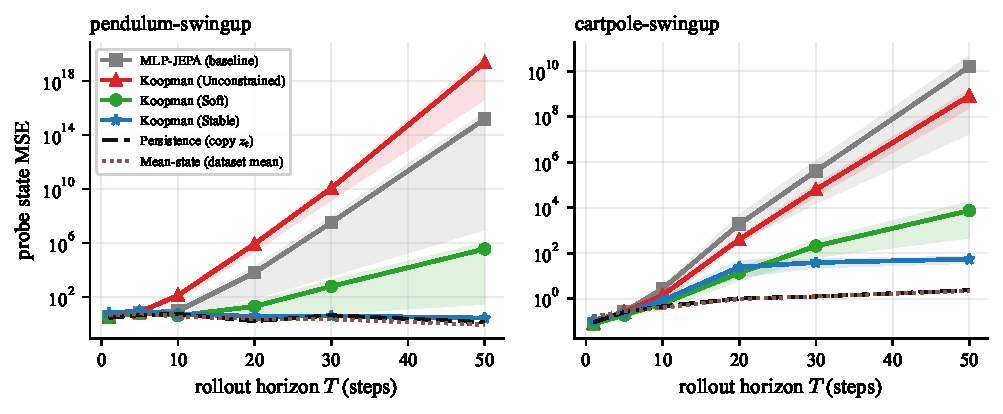
\includegraphics[width=\linewidth]{paper_figures/fig_compounding_controls.pdf}
    \caption{Error growth against horizon, with the two controls drawn as
    reference lines. \textbf{Left:} pendulum-swingup. \textbf{Right:}
    cartpole-swingup. Probe state MSE, mean over 10 seeds, log scale, with 95\%
    bootstrap intervals as shaded bands. Every series comes from the same
    evaluation pass, so the learned models and the controls share the
    checkpoint, the probe fit and the episodes.}
    \label{fig:compounding_controls}
\end{figure}

\begin{figure}[t]
    \centering
    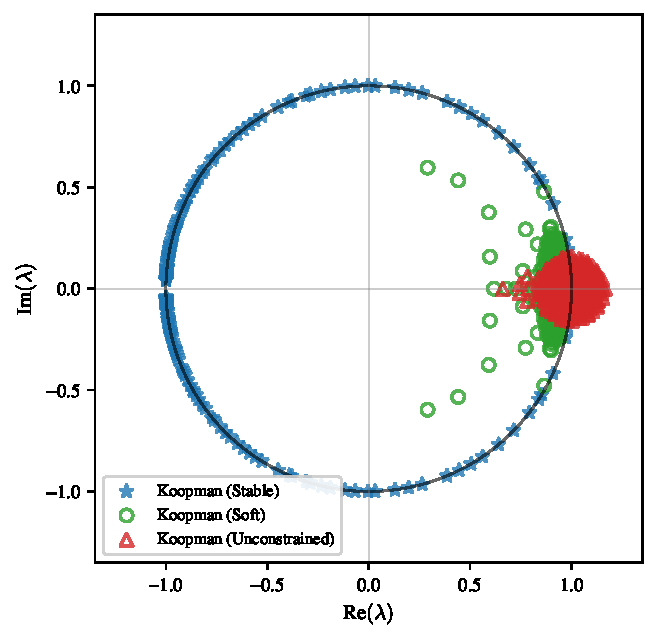
\includegraphics[width=0.4\linewidth]{paper_figures/fig_eigenvalues.pdf}
    \caption{The learned spectra are consistent with the error growth in
    Table~\ref{tab:drift}. Eigenvalues of each variant's operator on the complex
    plane, all latent dimensions, one representative seed on
    pendulum-swingup. Koopman~(Stable) lies exactly on the unit circle by
    construction, Koopman~(Soft) concentrates near it with a few eigenvalues
    beyond, and Koopman~(Unconstrained) drifts outside it.}
    \label{fig:eigenvalues}
\end{figure}

% =============================================================================
\section{What Produced Each Number}
\label{app:provenance}
% [new] DONE. Factual only. The third paragraph states the two protocol facts
% a reader needs in order to reproduce or to judge the comparisons, without
% narrating how they came to be known.
Every number in this paper comes from one of five result files, each produced by
a single evaluation job and released with the paper. Table~\ref{tab:combined},
Table~\ref{tab:retrieval}, Figure~\ref{fig:rho_sweep}, Figure~\ref{fig:degeneracy},
Figure~\ref{fig:compounding_controls} and the conditioning columns of
Table~\ref{tab:control} come from the diagnostics file, which covers both
environments and all four dynamics modules at clean backgrounds and full data.
The two tables of Appendix~\ref{app:full_results} come from the cells file,
which covers the same models across four backgrounds and four training data
fractions. Table~\ref{tab:drift} comes from the norm growth file, the solved
counts and gains of Table~\ref{tab:control} from the Riccati file, and
Table~\ref{tab:l2_ablation} from the two ablation files, one per prediction loss.

The evaluation environments are built from gymnasium~1.2.3, shimmy~2.0.0,
dm-control~1.0.36 and mujoco~3.4.0 on Python~3.11.9, with numpy~2.4.1 and
torch~2.9.1.

Two facts about the protocol matter for reading the tables. The held-out
episodes are collected under a uniformly random policy whose action stream is
seeded, so the evaluation set is determined by the seed and is identical across
the jobs above, which is what makes the two arms of Table~\ref{tab:l2_ablation}
comparable and what the matching dataset-mean control in that table records. And
the models were trained under an earlier build of the simulator stack than the
one they were evaluated under, so absolute error values are specific to this
evaluation set. Every comparison in the paper is between models scored on the
same episodes, which is the property the conclusions rest on. An evaluation set
regenerated from a collector is worth caching to disk instead.

\end{document}
